
\documentclass[11pt]{article}
%%%%%%%%%%%%%%%%%%%%%%%%%%%%%%%%
\usepackage{amsmath}
\usepackage{amsthm}
\usepackage{footnote}
\usepackage{fancyhdr}
\usepackage{amssymb}
\usepackage{tikz}
\usetikzlibrary{trees}


\theoremstyle{plain}
\newtheorem*{theorem*}{Theorem}
\newtheorem*{notation*}{Notation}
\newtheorem*{algorithm*}{Algorithm}
\newtheorem*{remark*}{Remark}
\newtheorem{theorem}{Theorem}[section]
\newtheorem{algorithm}{Algorithm}[section]
\newtheorem{axiom}[theorem]{Axiom}
\newtheorem{claim}[theorem]{Claim}
\newtheorem{corollary}[theorem]{Corollary}
\newtheorem{definition}[theorem]{Definition}
\newtheorem{example}[theorem]{Example}
\newtheorem{lemma}[theorem]{Lemma}
\newtheorem{notation}[theorem]{Notation}
\newtheorem{problem}[theorem]{Problem}
\newtheorem{proposition}[theorem]{Proposition}
\newtheorem{remark}[theorem]{Remark}
\newtheorem{summary}[theorem]{Summary}
\newtheorem{assumption}{Assumption}[section]

\DeclareMathOperator*{\argmax}{arg\,max}
\DeclareMathOperator*{\E}{\mathbb{E}}
\let\Pr\relax
\DeclareMathOperator*{\Pr}{\mathbb{P}}

\begin{document}

\title{Report for Independent Study\\
Streaming and Sketching Algorithms}
\author{Min Chen}
\date{\today}
\maketitle
\thispagestyle{fancy}
\lhead{Streaming and Sketching Algorithms}
\rhead{IUB Spring 2018}
\rfoot{Page \thepage}

\begin{abstract}
This is the report for an independent study with Prof. Qin Zhang at Indiana 
University Bloomington for the Spring Semester 2018. The independent study 
follows the outline of a course by Prof. Zhang: B669 Sublinear Algorithms for 
Big Data and focused on streaming and sketching algorithms. 
\end{abstract}
\pagebreak
\tableofcontents
\pagebreak

\part{Overview}
\paragraph{Introduction}
Sublinear algorithms have been studied to solve the problems of Big Data, 
and applied in various applications including internet traffic, social networks, 
etc. The author has been focused on streaming and sketching algorithms, 
which use small-space data structures that can be updated in a fast-moving 
stream of input. These algorithms are often sublinear in space, i.e. the entire 
data is too big to fit into the memory and we are trying to use limited memory 
along one or several passes over the data set to get the result. Most of the 
time, approximation and randomization techniques are applied, and we want 
to achieve a high accuracy in the approximated result.  

\paragraph{Outline}The report is structured in the following way: 
Part \ref{p:pre} talks about basic streaming models and definitions followed 
by commonly used probability tools in the analysis in this field including 
several inequalities for bounding the tail distributions. It also provides a 
summary of the widely used universal hash family and pseudo-random 
generator for sublinear space. The author tried to unify materials from 
several places and present in a easily understandable way with clear 
indications on the space usage and construction method. Part \ref{p:fm} 
focuses on frequency moments estimation and Part \ref{p:pq-hh} focuses on 
two related problems point query and heavy hitters. In these parts, the 
author unifies the algorithm from several lecture notes and organize them 
logically. Part \ref{p:sr-l0} introduces the important concept of 
$l_0$-sampling which is used as a tool for the graph sketches in Part 
\ref{p:graph}.


\paragraph{Materials and Resources }
There are several important sources that the author read and referenced 
when studying this topic and writing the report. 
\begin{itemize}
	\item Prof. Qin Zhang's course materials and 
	slides  \cite{zhang2017-slides}.The author followed these sets of slides as 
	a guidance for the major topics with a focus two parts, Sublinear in space 
	and Sublinear in communication. 
	\item Lecture Notes by Prof. Amit Chakrabarti  \cite{Cha2015-notes}. The 
	lecture notes provides detailed explanation, correctness proof and 
	discussion of several of the important streaming algorithms. 
	\item Course materials  by Prof. Jelani Nelson  \cite{Nel2015-web}. Prof. 
	Nelson from Harvard provides detailed lecture notes with Youtube videos 
	for recorded lectures. 
	\item Two papers by Ann, Guha and 
	McGregor  \cite{AGM2012-analyzing}  \cite{AGM2012-graph}. These 
	papers discuss a series of algorithms for graph sketch based on a sketch 
	algorithm of connectivity. 
	\item Text book: Probability and Computing by Mitzenmacher and 
	Upfal  \cite{MU-probability}. The book provides detailed explanation with 
	examples illustrating randomized algorithms used in computing. Some of 
	the preliminary probability tools are learnt and summarized from this book.
	\item Other notes, materials and papers used, will be acknowledged and 
	cited in later sections.
\end{itemize}

\pagebreak
\part{Preliminaries}
\label{p:pre}

This parts lays out some of the preliminaries as notational and technical 
foundations for other sections. Basic models and notations will be discussed 
first. Then some key equalities and inequalities in probability theory that is 
widely used in the analyses will be listed. Finally, since a lot of algorithms in 
this report use randomization and universal hash functions, The last section 
in this part will introduce some useful tools of hashing and 
pseudo-random generator by Nisan. 

\section{Basic Streaming Models and Notations}
\label{s:model}

This section introduces the basic streaming models, variations and 
notations\footnote{Materials are from Prof. Amit 
Chakrabarti  \cite{Cha2015-notes}}.

\subsection{Streaming Models}
Consider an input stream denoted by $\sigma$, which contains $m$ 
tokens/elements: $\sigma=\langle a_1, a_2, \dots, a_m\rangle$. The elements 
are drawn from the universe $[n] := {1, 2, \dots, n}$. 
Note the two important size parameters: the stream length, $m$, and the 
universe size, $n$. Some authors interchange these two symbols, in this 
report I consistently use m and n as defined here to follow the notes by 
Chakrabarti  \cite{Cha2015-notes}.

\begin{definition}
	The frequency vector $\textbf{f}=(f_1, f_2, \dots, f_n)$ for an input stream 
	$\sigma$ is defined as: 
	\[
	f_j=|\{i: a_i=j\}|
	\]
\end{definition}
In other words, $\sigma$ implicitly defines this vector $\textbf{f}$, and we 
are interested in computing some function of the form $\Phi(\textbf{f})$. 
While processing the stream, when we scan a token $j \in [n]$, we could just 
increment the frequency $f_j$. Thus, $\sigma$ can be thought of as a 
sequence of update instructions, updating the vector $\textbf{f}$. In general 
each element of the stream $a_i$ is in the form of $(j, c)$ where $j\in [n]$ 
and $c$ is some integer between $-L$ and $L$ (some upper bound and 
lower bound known upfront). This means that element $j$ is incremented by 
$c$, (where $c$ could be negative). 

Assuming that $\textbf{f}$ starts from the zero vector, upon receiving 
$a_i=(j,c)$, we update $f_j=f_j+c$. In this general case, the parameter $m$ 
will denote the maximum number of items at any point
of time i.e. 
\[
||\textbf{f}||_1 = \sum |f_i|\leq m
\]

\begin{definition}
Given an input stream $\sigma=\langle a_1, a_2, \dots, a_m\rangle$ and 
$a_i=(j, c)$ with frequency vector $\textbf{f}$ , we have the following basic 
stream models:
\begin{itemize}
	\item vanilla streaming model: $c=1$ for all $a_i=(j,c)$
	\item turnstile model: $c \in {-L,\dots,L}$ for all $a_i=(j,c)$
	\item cash register model: $c > 0$ for all $a_i=(j,c)$
	\item strict turnstile model: $ \textbf{f} \geq 0$ at all times
\end{itemize}
\end{definition}


\subsection{Space Goal} 

we want to achieve sub-linear spaces when 
processing the input stream, i.e. the number of bits used is sublinear in both 
$m$ and $n$. The space goal is $s=O(\log m + \log n)$ in general. 
Sometimes, the logarithmic space is impossible and we can only achieve
a space bound of the form $s = polylog(\min\{m, n\})$, where $f(n) = 
polylog(g(n))$ means that there exists a constant $c > 0$ such that $f (n) = 
O((\log g(n))^c)$  \cite{Cha2015-notes}.

\subsection{Quality of Approximation Algorithm}

 Randomization and 
approximation algorithms are often used to provide an estimate to the actual 
statistics $\phi(\sigma)$ of the data stream. The following two definitions by 
Chakrabarti will be used to evaluate the quality of the approximation:

\begin{definition}
\label{def:approximation}
		Let $A(\sigma)$ denote the output of a randomized streaming algorithm 
		A on input $\sigma$. Let $\phi(\sigma)$ be the function that 
		$A(\sigma)$ is supposed to compute. We say that the algorithm 
		($\epsilon$, $\delta$)-approximates  $\phi(\sigma)$ if:
		\[
		\Pr[|\frac{A(\sigma)}{\phi(\sigma)} - 1|>\epsilon]\leq \delta
		\]
		which sometimes is expressed as:
		\[
		\Pr[|A(\sigma)-\phi(\sigma)|>\epsilon\phi(\sigma)]\leq \delta
		\]
\end{definition}

\begin{definition}
\label{def:approximation-add}
	Let $A(\sigma)$ denote the output of a randomized streaming algorithm 
	A on input $\sigma$. Let $\phi(\sigma)$ be the function that $A(\sigma)$ 
	is supposed to compute. We say that the algorithm ($\epsilon$, 
	$\delta$)-additively-approximates  $\phi(\sigma)$ if:
	\[
	\Pr[|A(\sigma)-\phi(\sigma)|>\epsilon]\leq \delta
	\]
\end{definition}

Note that Definition  \ref{def:approximation} insists on a multiplicative 
approximation, which is stronger than the additive approximation in 
Definition  \ref{def:approximation-add}.

\subsection{Sketch and Linear Sketch}
\label{s:sketch}
Consider two data stream $\sigma_1$ and  $\sigma_2$, and we have ways to 
calculate some statistics $G(\cdot)$ for each stream. If we use $\sigma = 
\sigma_1\circ\sigma_2$ to denote the concatenation of the two streams, it 
would be handy to perform some simple calculation on $G(\sigma_1)$ and 
$G(\sigma_2)$ to get $G(\sigma)$. This leads to the following definition:

\begin{definition}
A data structure $DS(\sigma)$ computed in streaming fashion by processing 
a stream $\sigma$ is called a sketch if there is a space-efficient combining 
algorithm $COMB$ such that, for every two streams $\sigma_1$ and  
$\sigma_2$, we have
\[
COMB(DS(\sigma_1), DS(\sigma_2))=DS(\sigma_1\circ\sigma_2)
\]
\end{definition}
The simplest case is that the combining function is a linear function:

\begin{definition}
A sketching algorithm $sk$ is called a linear sketch if, for each stream 
$\sigma$ over a token universe $[n]$, $sk(\sigma)$ takes values in a vector 
space of dimension $l=l(n)$ and $sk(\sigma)$ s a linear function of 
$\textbf{f}(\sigma)$. 
\end{definition}
Notice that the combining algorithm for linear sketches is to simply add the 
sketches (in the appropriate vector space). For non-sketch algorithms on a 
stream, besides the difficulty to combine results of small streams to get 
results for concatenated stream, they also have the drawback that they often 
only work for vanilla streaming model instead of the more general turnstile
(or even strict turnstile) model. 

But the sketch algorithms work for turnstile model. If the arrival of a token 
$j$ in the vanilla model causes us to add a vector $\textbf{v}_j$ to the 
sketch, then an update $(j,c)$ in the turnstile model is handled by adding 
$c\textbf{v}_j$ to the sketch: this handles both cases $c\geq0$ and $c<0$.

Nelson provides another explanation using the matrix notation:
\begin{quotation}
	The common/only technique for designing turnstile algorithms is 
	\textbf{linear sketching}. The idea is to maintain in memory $y = \Pi x$, 
	where $\Pi \in \mathbb{R}^{m \times n}$, a matrix that is short and fat. We 
	care that $m<n$, usually much smaller. We can see that $y$ is 
	$m$-dimensional so we can store it efficiently but what about $\Pi$? If we 
	need to store the whole $\Pi$ in memory this will not lead to a better 
	algorithm in terms of space. So, there are two common ways in 
	constructing and storing $\Pi$. The one is that $\Pi$ is deterministic and 
	so we can easily compute $\Pi_{ij}$ without keeping the whole matrix in 
	memory. The other way is that $\Pi$ is defined by $k$-wise independent 
	hash functions for some small $k$ or using Nisan's PRG (in 
	Section  \ref{s:hashprg}), so we can afford storing the hash 
	functions and computing $\Pi_{ij}$.	
	
	Let's see now how updates happen when we have a linear sketch. Let 
	$\Pi^i$ be the $i$-th column of the matrix $\Pi$. Then $\Pi_x = \sum_{i=1}^n 
	\Pi^i x_i$. So by storing $y = \Pi x$ when the update $(i,\Delta)$ comes we 
	have that the new $y$ equals $\Pi(x+ \Delta e_i) = \Pi x + \Delta \Pi^i$. 
	Observe that the first term is the old $y$ and the second term is just some 
	multiple of the $i$-th column of $\Pi$. This means that if I can tell which is 
	the $i$-th column of $\Pi$ in small space I can also perform updates in 
	small space.
\end{quotation}

\section{Useful Probability Tools and Techniques}
This section will list several of the useful tools in Probability Theory that used 
to analyse algorithms in later sections\footnote{Materials are from Prof. 
Jelani Nelson  \cite{Nel2015-web}, Prof. Qin Zhang's 
slides  \cite{zhang2017-slides} and Mitzenmacher and 
Upfal's book  \cite{MU-probability} }.

\begin{lemma}[Union Bound]
\label{le:unionbound}
	For a countable sets events $A_1$, $A_2$, $A_3$, ..., we have:
	\[
	\Pr(\bigcup_i A_i)\leq \sum_i \Pr(A_i)
	\]
\end{lemma}
One proof could be done by applying countable additivity and monotonicity 
of the probability measure, the detail is omitted here. 

\begin{lemma} [Linearity of Expectation]
\label{le:linearityofe}
	Let $X_i$ be random variables, 
	\[
	\E(\sum_i^{\infty} X_i)=\sum_i^{\infty} \E X_i
	\]
\end{lemma}

\begin{lemma} [Markov]
\label{le:markov}
Let $X$ be a non-negative random variable, $\forall \lambda>0$, 
\[
\Pr(X>\lambda)<\frac{\E X}{\lambda}
\]
\end{lemma}
\begin{proof}
	Consider the Indicator random variable: $I_{\{X>\lambda\}}$,  $\E 
	I_{\{X>\lambda\}}=\E I_{\{X/\lambda>1\}}<\E(X/\lambda)=\frac{\E 
	X}{\lambda}$. Hence, $\Pr(X>\lambda)=\E 
	I_{\{X>\lambda\}}<\frac{\E X}{\lambda}$
\end{proof}

\begin{lemma}[Chebyshev]
	\label{le:chebyshev}
	$\forall \lambda>0$ and random variable $X$,
	\[
	 \Pr(|X-\E X| > \lambda)<\frac{\E(X-\E 
	 X)^2}{\lambda^2}=\frac{Var(X)}{\lambda^2}
	\]
\end{lemma}

\begin{proof}
	$\Pr(|X-\E X|>\lambda)=\Pr((X-\E X)^2>\lambda^2)$. Then the result 
	follows Markov (Lemma  \ref{le:markov})
\end{proof}

Moreover, Chebyshev can be generalized to :

\begin{lemma}
\[
\forall p>0, \forall \lambda>0, \Pr(|X-\E X| > \lambda)<\frac{\E(X-\E 
	X)^p}{\lambda^p}
\]
\end{lemma}

\begin{theorem}[Chernoff]
\label{th:chernoff}
	$X_1,\ldots, X_n$ are independent random variables, where $X_i\in \{0,1\}$. 
	Let $X=\sum_{i}{X_i}$, $\mu = \E X$ then the following Chernoff bounds 
	hold: 
	\begin{enumerate}
		\item 	for any $\delta>0$
		\begin{equation}
		\label{eq:chernoff1}
		\Pr(X>(1+\delta )\mu )<\left({\frac {e^{\delta }}{(1+\delta )^{(1+\delta 
					)}}}\right)^{\mu }
		\end{equation}
		
		\item 	for any $0<\delta\leq 1$
		\begin{equation}
		\label{eq:chernoff2}
		\Pr(X<(1-\delta )\mu )<\left({\frac {e^{-\delta }}{(1-\delta 
		)^{(1-\delta )}}}\right)^{\mu }
		\end{equation}
		
		\begin{equation}
		\label{eq:chernoff3}
		\Pr(X\leq (1-\delta )\mu )\leq e^{-{\frac {\delta ^{2}\mu }{2}}}
		\end{equation}
		
		\begin{equation}
		\label{eq:chernoff4}
		\Pr(X\geq (1+\delta )\mu )\leq e^{-{\frac {\delta ^{2}\mu }{3}}}
		\end{equation}
			
	\end{enumerate}
\end{theorem}
The proof of Theorem  \ref{th:chernoff} can be found in Chapter 4 of the 
book Probability and Computing by Mitzenmacher and 
Upfal  \cite{MU-probability}. Notice that Equation  \ref{eq:chernoff1} and 
Equation  \ref{eq:chernoff2} are stronger than Equation  \ref{eq:chernoff3} 
and Equation  \ref{eq:chernoff4}, however, the latter have a simpler form 
thus easier to use and are often sufficient in the analysis. We could also 
combine Equation  \ref{eq:chernoff3} and Equation  \ref{eq:chernoff4} 
together and resulting in Corollary  \ref{co:chernoff}, which is widely used in 
general.

\begin{corollary}
\label{co:chernoff}
	$X_1,\ldots, X_n$ are independent random variables, where $X_i\in \{0,1\}$. 
Let $X=\sum_{i}{X_i}$, $\mu = \E X$, for any $0<\delta\leq 1$:
\[
\Pr(|X- \mu| \geq \delta \mu) \leq 2e^{- \delta^2 \mu/3}
\]
\end{corollary}


\section{Universal Hashing and Derandomization}
\label{s:hashprg}

Randomized algorithms are widely used in these topics and this section will 
list several of the important definitions regarding universal hashing and 
pseudo-randomness, which turn out to be an important component in the 
analyses of algorithms. 

\subsection{Universal Hash Family}
\begin{definition} 
\label{def:2wise}
A family $\mathcal{H}$ of functions mapping $[a]$ to 
$[b]$ forms a $2$-universal hash family (is $2$-wise independent) if $\forall 
j_1,, j_2 \in [b]$ and $\forall$ distinct $i_1,i_2 \in [a]$,
	$$P_{h \in \mathcal{H}}(h(i_1) = j_1 \wedge h(i_2) = j_2) = 
	1/b^2$$ 
\end{definition}
%\begin{remark}
%Definition  \ref{def:2wise} basically states that for a \textbf{randomly} 
%selected hash function from the $2$-universal hash family, the hash value 
%of 
%two distinct items, which are two random variables, are independent. 
%\end{remark}
%\begin{remark}
%$2$-wise independence implies uniformity (which is weaker), i.e. 
%$$P_{h \in \mathcal{H}}(h(i) = j ) = 1/b$$ 
%\end{remark}

To generalize $2$-universal hash family to  $k$-universal hash family, we 
have Definition  \ref{def:kwise}:
\begin{definition} 
\label{def:kwise}
A family $\mathcal{H}$ of functions mapping $[a]$ to 
$[b]$ forms a $k$-universal hash family (is $k$-wise independent) if $\forall 
j_1, \ldots, j_k \in [b]$ and $\forall$ 
distinct $i_1, \ldots, i_k \in [a]$,
	$$P_{h \in \mathcal{H}}(h(i_1) = j_1 \wedge \ldots \wedge h(i_k) = j_k) = 
	1/b^k$$ 
\end{definition}
\begin{remark}
	Definition  \ref{def:kwise} basically states that for a \textbf{randomly} 
	selected hash function from the $k$-universal hash family, the hash value 
	of $k$ distinct items, which are $k$ random variables, are independent. 
	However, for more than $k$ such random variables, independence is not 
	guaranteed.  
\end{remark}
\begin{remark}
	$k$-wise independence implies uniformity (which is weaker), i.e. 
	$$P_{h \in \mathcal{H}}(h(i_1) = h(i_2)=\dots=h(i_k  ) = 1/b^{k-1}$$ 
\end{remark}

The use of universal hash families is well-illustrated by the definition: 
sometimes we do not need full independence, $k$-wise independence is 
sufficient. For example, consider random variables $X_i$, $i\in{1,2,\dots,r}$. 
\[
Var(\sum X_i)=\sum Var(X_i)+2\sum_i\sum_j Cov(X_i, X_j)=\sum Var(X_i)
\]
The first equality is by definition and the second equality holds when $X_i$'s 
are 2-wise independent. 

\paragraph{Construction and Representation}
The construction of $k$-universal hash family could be done by using 
random polynomials over finite fields. We could generate a $k$-universal 
hash family from $[l]$ to $[l]$ in the following steps: 
\begin{enumerate}
	\item Let $F_l$ be a finite field of $l$ elements
	\item Pick $c_0, c_1, \dots, c_{l-1}\in F_l$ uniformly at random. 
	\item Define $h(x)=\sum_{i=0}^{l-1}c_ix^i$, where the multiplication and 
	addition are within the field $F_l$
	\item $\mathcal{H}=\{h(x)=\sum_{i=0}^{l-1}c_ix^i: \quad c_0, c_1,\dots, 
	c_{l-1}\in F_l\}$ is the family needed
\end{enumerate}
\begin{remark} Observations from the construction:
	\begin{enumerate} 
		\item $\mathcal{H}$ has size $l^k$ by construction
		\item To represent $\mathcal{H}$, we need $k\log l$ random bits: $\log 
		l$ bits each for $c_0, c_1, \dots, c_{l-1}$
		\item If in general we need $k$-universal hash family from $[l]$ to $[g]$ 
		where $g<l$, we just need to add one modular operation to $h$, i.e. 
		\[
		h(x)=(\sum_{i=0}^{l-1}c_ix^i) \mod g 
		\]
	\end{enumerate}
\end{remark}
\begin{example}
	To draw a hash function from a 3-universal family from $[n]$ to $[5]$, 
	assuming $n$ is a prime number. Use the field $F_l=\{0,1,\dots, n-1\}$ and 
	randomly select three numbers $a$, $b$, $c$ uniformly from $F_l$. Then 
	the hash function we need is 
	\[
	h(x)=((a+bx+cx^2)\mod n) \mod 5
	\]
	To store $h(x)$, we need to store $a$, $b$, and $c$, that is $3\log n$ 
	bits, i.e. $O(\log n)$ bits
\end{example}

\subsection{Nisan's Pseudo-random Generator (PRG)}

There are times that $k$-wise independence is insufficient for the algorithm 
and one may need full-randomness in order to get the desired result. That is 
when Pseudo-random Generator (PRG) is needed. 

Definition  \ref{def:prg} and Remark  \ref{re:prg} are copied from Prof. Yuan 
Zhou's lecture notes in the course A Theorist’s Toolkit Fall 
2016  \cite{Zhou-theory}:

\begin{definition}
\label{def:prg}
Let $C$ be a class of functions of $f : \{0, 1\}^n \rightarrow \{0, 1\}$.  
$G : \{0, 1\}^l \rightarrow \{0, 1\}^n$ with $(l < n)$ is an $\epsilon$-PRG for 
$C$ with seed length $l$ if
\[
\forall f\in C \qquad |\Pr_{r\sim\{0,1\}^n}[f(r)=1] -  
\Pr_{s\sim\{0,1\}^l}[f(G(s))=1]|<\epsilon 
\]
Then, we say that $G$ $\epsilon$-fools $C$.  Ideally, $G(s)$ should be 
deterministically computable in polynomial
time.
\end{definition}
\begin{remark}
\label{re:prg}
	Functions in $C$ can not distinguish between distribution 
	$\{G(s)\}_{s\sim\{0,1\}}$ and uniform distribution $\{0, 1\}^n$. However, 
	$\{G(s)\} $ has a much smaller support. 
\end{remark}

The author will in particular focus on one PRG provided by 
Nisan  \cite{Nisan1990-prg}, which is for space-bounded computations. This 
PRG will be used in this report in Section  \ref{s:norm-stabled} when 
discussing estimating $l_p$ norms using stable distribution. The initial work 
is done by Piotr Indyk  \cite{Indyk2006-prg}. In the following paragraphs, I 
will first present two descriptions of this Pseudo-random Generator one by 
Prof. Indyk and the other by Prof. Nelson in his lecture 
notes  \cite{Nel2015-web}.

\paragraph{Indyk's Version}
There exists a PRG $G$ for SPACE(S) with parameter $\epsilon=2^{−O(S)}$ 
such that:
\begin{itemize}
	\item $G$ expands $O(S \log R)$ bits into $O(R)$ bits
	\item $G$ requires only $O(S)$ bits of storage (in addition to its random 
	input)
	\item any length $O(S)$ chunk of $G(x)$ can be computed using $O(\log 
	R)$ arithmetic 	operations on $O(S)$-bit words
\end{itemize}
Note that in our cases, $S=O(\log n)$

\paragraph{Nelson's Version}(Copied from his lecture 
notes  \cite{Nel2015-web}):

\begin{quotation}
A {\em branching program} can be described with a grid of nodes 
representing different states of the program---we can think of it as a DFA. 
The program starts at an initial node which is not part of the grid. At each 
step, the program reads $S$ bits of input, reflecting the fact that space is 
bounded by $S$, and makes a decision about which node in the subsequent 
column of the grid to jump to. After $R$ steps (number of columns in the 
grid), the final node visited by the program represents the outcome. The 
entire input, which can be represented as a length-$RS$ bit string, induces a 
distribution over the final states. Our goal is to generate the input string 
using fewer ($\ll RS$) random bits such that the original distribution over 
final states is well preserved. The following theorem addresses this goal.

\begin{theorem} (\cite{Nisan1990-prg}) \label{thm:nisan}
	There exists $h:\{0,1\}^{t}\rightarrow\{0,1\}^{RS}$ for $t=O(S\lg R)$ such 
	that 
	\begin{equation*}
	\left| P_{x\sim U(\{0,1\}^{RS})}\left\{ f(B(x))=1 \right\} -P_{y\sim 
		U(\{0,1\}^{t})}\left\{ f(B(h(y)))=1 \right\} \right| \le \frac{1}{2^{S}}.
	\end{equation*}
	for any branching program $B$ and any function 
	$f:\{0,1\}^{S}\rightarrow\{0,1\}$. 
\end{theorem}

In other words, such function $h$ can simulate the input to the branching 
program with only $t$ random bits such that it is almost impossible to 
discriminate the outcome of the simulated program from that of the original 
program.

What does such a function look like? We start by taking a random sample 
$x$ from $\{0,1\}^S$. Then we place $x$ at the root and repeat the following 
procedure to create a complete binary tree. At each node, create two children 
and copy the string over to the left child. For the right child, use a random 
2-wise independent hash function $h_j:[2^S]\rightarrow[2^S]$ chosen for the 
corresponding level of the tree and record the result of the hash. Once we 
reach $R$ levels, output the concatenation of all leaves, which is a 
length-$RS$ bit string. To illustrate, the first few levels of our tree would look 
like:

\begin{center}
	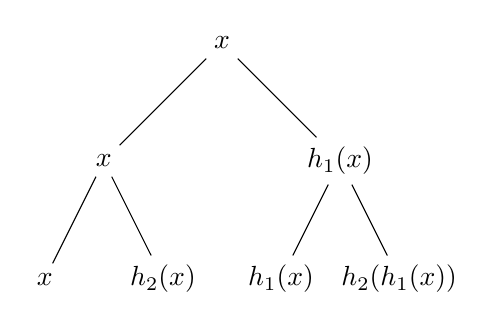
\begin{tikzpicture}[level distance=1.5cm,
	level 1/.style={sibling distance=3cm},
	level 2/.style={sibling distance=1.5cm}]
	\node {$x$}
	child {node {$x$}
		child {node {$x$}}
		child {node {$h_2(x)$}}
	}
	child {node {$h_1(x)$}
		child {node {$h_1(x)$}}
		child {node {$h_2(h_1(x))$}}
	};
	\end{tikzpicture}
\end{center}

Since each hash function requires $S$ random bits and there are $\lg R$ 
levels in the tree, this function uses $O(S\lg R)$ bits total. We will not 
discuss why this function satisfies the condition in Theorem  \ref{thm:nisan}
\end{quotation}

\begin{summary}[Space of Nisan]
	To summarize the two versions, if we need some random hash function 
	$h:[n]\rightarrow[m]$, which needs $R=n\log m $ bits. By using Nisan to 
	generate $h$, it blows up the space by $\log R$. Therefore, the total space 
	is:
	\[
	n\log m \cdot \log R = n\log m \log(n\log m) \approx \log n \cdot n\log m 
	\]
	This illustrates what is often mentioned by the lecture notes and paper 
	that ``Nisan blows space up by a factor of $\log n$''.
\end{summary}

\pagebreak
\part{Frequency Moments}
\label{p:fm}

Recall in a stream $\sigma$ where elements are from $[n]$. The frequency 
vector $\textbf{f}=\textbf{f}(\sigma)=(f_1, f_2, \dots, f_n)$. Then the $k$th 
frequency moment of the stream $F_k(\sigma)$ or simply $F_k$ is defined as 
follows:
\[
F_k:=\sum_{j=1}^n f_j^k=||\textbf{f}||_k^k
\]
where $||\textbf{f}||_k$ is the $k$-norm of \textbf{f} with 
$||\textbf{f}||_k:=(\sum_{j\in [n]} f_j^k)^{1/k}$

Notice that this definition does not only hold for $k$ being positive integers, 
it holds for positive real numbers. Moreover, If we set a convention that 
$0^0=0$, then $F_0=\sum_{j:f_j>0} f_j^0=|\{j:f_j>0\}|$, which is the number of 
distinct elements in the stream. 

In this part, We will first introduce several algorithms estimating number of 
distinct elements, $F_0$. Then we will discuss the algorithms for $F_p$ in 
several cases: $p=2$, $0<p<2$ and $p>2$. Some of the algorithms work 
only for vanilla streaming model but some work for turnstile model. 

Below are some results by researchers in this field
\begin{itemize} 
	\item $0 \leq p \leq 2, poly(\frac{logn}{\epsilon})$ space is achievable for 
	$(1+\epsilon)$ approximation with $\frac{2}{3}$ success probability 
	\cite{AMS99,Indyk2006-prg}.
	\item For $p >2$ then we need exactly $\Theta(n^{1-\frac{2}{p}} 
	poly(\frac{logn}{\epsilon}))$ bits of space for $(1+\epsilon)$ space with 
	$\frac{2}{3}$ success probability \cite{Bar-Yossef04,IndykW05}.
\end{itemize}




\section{Number of Distinct Elements ($F_0$)}
This section focuses on estimating the number of distinct elements of a data 
stream, i.e $F_0$. 

\subsection{Idealized Algorithm: FM}

This algorithm was originally by Flajolet and Martin  \cite{Flajolet85-f0} and 
presented in Nelson's lecture notes.

\begin{algorithm}[FM]
\label{al:fm}
In a vanilla streaming model with stream $\sigma$
\begin{enumerate}
	\item Pick random function $h: [n] \to [0,1]$ (idealized, since we can't 
	actually nicely store this and precision of real number is problematic)
	\item Maintain counter $X = \min_{i \in \sigma} h(i)$
	\item Output $1/X - 1$
\end{enumerate}
\end{algorithm}

\paragraph{Intuition} The intuition behind the algorithm goes as follows: if 
we have $n$ distinct elements, by random hash function $h$, the $n$ 
different hash value are likely to spread out over interval $(0,1)$, splitting the 
interval into $n+1$ small intervals. The minimal counter $X$ will be in 
expectation equal to $\frac{1}{n+1}$ (the end of the first small interval), 
hence  $1/X - 1$ is an estimate for $n$.

\paragraph{Analysis} $X$ is a random variable that's the minimum of $t$ 
i.i.d $Unif(0,1)$ r.v.s. We could show the following claims: 
\begin{enumerate}
	\item $\mathbb E X = \frac{1}{t+1}$.
	\item $\mathbb E X^2 = \frac{2}{(t+1)(t+2)}$
	\item $Var[X] = \frac{t}{(t+1)^2(t+2)}$
\end{enumerate}
Therefore, the estimator $1/X - 1$ here is unbiased, however, the variance is 
kind of large. (from Section  \ref{s:model}, we want some 	($\epsilon$, 
$\delta$)-approximation). We could average together multiple estimates from 
FM to reduce variance: 

\begin{algorithm}[FM+]
	\label{al:fm+}
	In a vanilla streaming model with stream $\sigma$
	\begin{enumerate}
\item Instantiate $q = 1/\epsilon^2\eta$ FMs independently
\item Let $X_i$ come from FM$_i$.
\item Output $1/Z - 1$, where $Z = \frac1q \sum_i X_i$.
	\end{enumerate}
\end{algorithm}

\paragraph{Intuition and Analysis}
The intuition behind FM+ is that averaging $q$ FM counters will reduce the 
variance. In fact, we have $\mathbb E(Z) = \frac{1}{t+1}$, and $Var(Z) = \frac 
1q \frac{t}{(t+1)^2(t+2)} < \frac{1}{q(t+1)^2}$. Then by Chebyshev 
(Lemma  \ref{le:chebyshev}), we could show that $P(|Z - \frac{1}{t+1}| > 
\frac{\epsilon}{t+1}) < \eta$, which implies that $P(| (\frac{1}{Z} - 1) - t | > 
O(\epsilon)t) < \eta$.  This is an $(O(1)$, 
$\eta$)-approximation. We could improve this further by using the 
so-called \textbf{Median Trick}:

\begin{algorithm}[FM++]
	\label{al:fm++}
	In a vanilla streaming model with stream $\sigma$
	\begin{enumerate}
	\item Instantiate $s = \lceil 36 \ln (2 / \delta) \rceil$ independent copies of 
	FM+ with $\eta = 1/3$.
	\item Output the median $\widehat{t}$ of $\{ 1/Z_j - 1 \}_{j=1}^s$ where 
	$Z_j$ is from the $j$th copy of FM+.
	\end{enumerate}
\end{algorithm}

\paragraph{Intuition and Analysis}
The intuition behind this improvement is that, we could take a bunch of 
estimator from FM+, use the median as a new estimator. To make the median 
fail, at least half of the estimators would fail and that is some small 
probability $\epsilon$ if we choose sufficient large number of estimators. The 
analysis is an application of Chernoff bound (Theorem  \ref{th:chernoff}), 
and one could show that $P(|\widehat{t} - t| > \epsilon t) < \delta$, which is 
the desired ($\epsilon$, $\delta$)-approximation we want. 

\paragraph{Space}
The final space required, ignoring $h$, is $O(\frac{\lg(1/\delta)}{\epsilon^2})$ 
for $O(\lg (1/\delta))$ copies of FM+ that require $O(1/\epsilon^2)$ space 
each.

\begin{remark}
The series of FM algorithms provides some idea of estimating $F_0$, and we 
can actually achieve ($\epsilon$, $\delta$)-approximation using space 
$O(\frac{\lg(1/\delta)}{\epsilon^2})$. However, since we cannot efficient store 
$h$ and also $h$ maps to real numbers on $(0,1)$, this algorithm is only 
idealized.
\end{remark}

\subsection{Non-idealized Version of FM: AMS-For-$F_0$}

To resolve the idealized part of FM algorithm, this subsection presents the 
algorithm by Alon, Matias and Szegedy  \cite{AMS99}. These authors also 
discussed other algorithms for different problems in the same paper, 
therefore we refer to this as AMS-For-$F_0$\footnote{Materials are from 
Prof. Jelani Nelson  \cite{Nel2015-web}, Prof. Qin Zhang's 
slides  \cite{zhang2017-slides} and Prof. Amit 
Chakrabarti  \cite{Cha2015-notes}}.

\begin{definition}
\label{def:zeros}
For an integer $p > 0$, let $zeros(p)$ denote the number of zeros that the 
binary representation of $p$ ends with. Formally,
\[
zeros(p) = \max\{i : p\equiv0\mod 2^i \}.
\]
\end{definition}

\begin{algorithm}[AMS-For-$F_0$] Given a stream $\sigma$ assuming 
vanilla streaming model: 
\label{al:amsf0}
	\begin{enumerate}
		\item Choose a random hash function $h : [n] \rightarrow[n]$ from a 
		2-universal family. Set $z = 0$
		\item For each new coming item $j$,if $zeros(h(j)) > z$, 
		then set $z = zeros(h(j))$
		\item Output $2^{z+0.5}$
	\end{enumerate}
\end{algorithm}

\paragraph{Intuition}The basic intuition here is that due to randomness of 
$h$, for $d$ distinct elements, $zeros(h(j))$ should be ``spread out'' 
uniformly between 0 and $\log d$ (just like $\min h(i)$ in FM). Then there is 1 
out of $d$ element have $zeros(h(j))\geq\log d$. We also do not expect any 
tokens to have $zeros(h(j))\gg\log d$. Therefore, we maintaining the largest  
$zeros(h(j))$ in $z$, will roughly estimate $\log d$. 

\paragraph{Analysis} Instead of the detailed analysis, which can be found in 
Chakrabarti's notes  \cite{Cha2015-notes}, we will outline the important 
steps: 
\begin{enumerate}
	\item let $X_{r,j}$ be an indicator random variable for the event 
	$zeros(h(j))\geq r$ and let $Y_r = \sum_{j:f_j>0}X_{j,r}$. Denote the value 
	of $z$ at the end of algorithm by $t$, then $\hat{d}=2^{t+0.5}$
	\item By randomness of $h$ and pairwise independence of $X_{r,j}$ (since 
	$h$ is from 2-universal family), we have 
	$\E[X_{r,j}]=\frac{1}{2^r}$, 
	$\E[Y_{r}]=\frac{d}{2^r}$, 
	and $Var[Y_{r}]\leq\frac{d}{2^r}$
	\item By Markov’s and Chebyshev’s inequalities respectively, we have 
	$\Pr(t\geq r)=\Pr(Y_r>0)\leq\frac{d}{2^r}$,  and $\Pr(t\leq 
	r-1)=\Pr(Y_r=0)\leq\frac{2^r}{d}$
	\item These imply that $\Pr(\hat{d}\geq5d)\leq \sqrt{2}/5$ and  
	$\Pr(\hat{d}\leq d/5)\leq \sqrt{2}/5$ 
	\item Then we know that 
	$\Pr[|\hat{d}-d|>5d]\leq \sqrt{2}/5<1/3$. 
\end{enumerate}
Besides, we used $\log n$ bits space to store $h$ according to 
Section  \ref{s:hashprg} and $\log\log n $bits to store $z$, hence total space 
is $O(\log n)$. However, this is only $O(1)$-approximation. 

\paragraph{Median Trick}
We could apply the median trick again to initiate $k=\Theta(\log(1/\delta))$ 
independent copies of this algorithm and output the median of the $k$ 
answers. Chernoff bounds will ensure that the failure probability is bounded 
by $\delta$. In this case the space is $O(\log(1/\delta)\log n)$. These result is 
summarized in the following theorem:
\begin{theorem}
The number of distinct elements can be $(O(1),\delta)$-approximated using 
$O(\log(1/\delta)\log n)$ bits.
\end{theorem}

\subsection{An Improved Algorithm: BJKST}
The AMS-For-$F_0$ algorithm only provides an $(O(1),\delta)$-approximation 
to the number of distinct elements and we want to achieve 
$(\epsilon,\delta)$-approximation. An improved algorithm presented in the 
subsection is due to Bar-Yossef, Jayram, Kumar,
Sivakumar and Trevisan  \cite{BJKST02} \footnote{Materials are from Prof. 
Qin Zhang's slides  \cite{zhang2017-slides} and Prof. Amit 
Chakrabarti \cite{Cha2015-notes}}.

\begin{algorithm}[BJKST] Given a stream $\sigma$ assuming 
	vanilla streaming model. The values $b$ and $c$ are universal constants 
	that will be determined later, based on the desired guarantees
	on the algorithm’s estimate. $zeros()$ is defined in 
	Definition  \ref{def:zeros}
	\label{al:bjkst}
	\begin{enumerate}
		\item Choose a random hash function $h : [n] \rightarrow[n]$ from a 
		2-universal family. Set $z = 0$, $B=\phi$
		\item Choose another random hash function $g : [n] 
		\rightarrow[b\epsilon^{-4}\log^2 n]$ from a 2-universal family.
		\item For each new coming item $j$,if $zeros(h(j)) > z$, then 
		\begin{enumerate}
			\item set $B=B\cup\{g(j),zeros(h(j))\}$
			\item if $|B|>c/\epsilon^2$, then set $z=z + 1$ and remove all 
			$(\alpha, \beta)$ in $B$ with $\beta < z$. 
		\end{enumerate}
		\item Output $|B|2^{z}$
	\end{enumerate}
\end{algorithm}

\paragraph{Intuition} The following intuition is in Chakrabarti's 
notes  \cite{Cha2015-notes}.
\begin{quotation}
	Intuitively, this algorithm is a refined version of the AMS-For-$F_0$ 
	Algorithm. This time, rather than simply tracking the maximum value of 
	$zeros(h(j))$ in the stream, we try to determine the size of the bucket $B$ 
	consisting of all tokens $j$ with $zeros(h(j)) > z$, Of the $d$ distinct 
	tokens in the stream, we expect $d/2^z$ to fall into this bucket.
	Therefore $|B|2^{z}$ should be a good estimate for d.
	
	We want $B$ to be small so that we can store enough information 
	(remember, we are trying to save space) to track
	$|B|$ accurately. At the same time, we want $B$ to be large so that the 
	estimate we produce is accurate enough. It turns
	out that letting $B$ grow to about $O(1/\epsilon)$ in size is the right 
	tradeoff. Finally, as a space-saving trick, the algorithm does not store the 
	actual tokens in B but only their hash values under $g$, together with the 
	value of $zeros(h(j))$ that is needed to remove the appropriate elements 
	from $B$ when $B$ must be shrunk.
\end{quotation}

\paragraph{Space}
The algorithm needs to store $h$, $g$, $z$ and $B$. According to 
Section  \ref{s:hashprg}, $h$ needs $\log n$ bits, $g$ needs at most the 
same space. $B$ has size at most $O(1/\epsilon^2)$, each item in $B$ 
requires $\log (b\epsilon^{-4}\log^2 n)+\log\log n=O(\log(1/\epsilon)+\log\log 
n)$ bits. Hence the total space requirement is 
$O(1/\epsilon^2(\log(1/\epsilon)+\log\log n)+\log n)$. 

\paragraph{Analysis} Without providing details the of analysis (which could 
be found in Chakrabarti's 
notes  \cite{Cha2015-notes}), one could show that the above algorithm 
$(\epsilon,1/3)$-approximates $d$. As before, by using the median trick, we 
can improve this to an $(\epsilon,\delta)$-approximation with an additional 
factor of $\log(1/\delta)$ in the space requirements, which lead to Theorem~

\begin{theorem}
	\label{th:bjkst}
	The number of distinct elements can be $(\epsilon,\delta)$-approximated 
	using  $O(\frac{1}{\delta\epsilon^2}(\log(1/\epsilon)+\log\log 
	n)+\frac{1}{\delta}\log n)$ bits.
\end{theorem}

\subsection{Nelson's Algorithm with Geometric Sampling}
In this section, I present an algorithm with geometric sampling provided by 
Nelson  \cite{Nel2015-web}. 

\begin{algorithm}
Consider an trivial solution algorithm TS, which stores first $C/\epsilon^2$ 
distinct elements. This is correct if $d \leq C/\epsilon^2$.
\begin{enumerate}
	\item Instantiate TS$_0$, \dots, TS$_{\lg n}$
	\item Pick $g : [n] \to [n]$ from 2-universal family
	\item Feed $i$ to TS$_{lsb(g(i))}$, where $lsb$ is the least significant bit of 
	a number
	\item Output $2^{j+1}\cdot output(TS_j)$, where $t/2^{j+1}\approx 
	1/\epsilon^2$
\end{enumerate}
\end{algorithm}


\paragraph{Intuition and Analysis}
This algorithm is somewhat similar to BJKST, each TS only keeps number of 
distinct elements up to $C/\epsilon^2$, which is similar to the bucket $B$ in 
BJKST. Let $d_j$ be the number of distinct elements hashed by $g$ to 
TS$_j$. Then $\E d_j = d/2^{j+1} = Q_j$. By Chebyshev $d_j = Q_j \pm 
O(\sqrt{Q_j})$ with good probability. This equals $(1 \pm O(\epsilon)) Q_j$ if 
$Q_j \geq 1/\epsilon^2$. The Final space: $\frac{C}{\epsilon^2} (\lg n)^2 = 
O(\frac 1{\epsilon^2} \lg^2 
n)$ bits.

\paragraph{Optimality of $F_0$ Algorithms}
It is known that the algorithms we presented here are not the optimal for 
number of distinct elements in vanilla streaming model, we address this by 
the following remark. 
\begin{remark}
\label{re:f0optimal}
It is known that space $O(1/\epsilon^2 + \log n)$ is achievable  \cite{KNW10}, 
and furthermore this is optimal  \cite{Woodruff04}  \cite{AMS99}.
\end{remark}

\subsection{A Linear Sketch for $F_0$}
 
Although we have discussed several algorithms for distinct elements, and 
Remark  \ref{re:f0optimal} states that lower bound has been proved and 
achieved, we restrict the model to be vanilla streaming. If we allow deletions, 
the previous algorithms do not work. In this subsection, we present a linear 
sketch for estimating number of distinct elements. It will not be as efficient in 
space as the optimal but allow deletions in the stream. We will assume that 
we are in strict turnstile model (i.e. there is deletion but $\textbf{f}\geq 0$ all 
the time)\footnote{Materials are from Prof. Qin Zhang's 
slides  \cite{zhang2017-slides} and Prof. Piotr Indyk's 
slides  \cite{indyk07-web}}.

\paragraph{General Idea}
The idea of the algorithm is that for a given $T>0$, provide an algorithm
which, with probability $1-\delta$ such that:
\begin{itemize}
	\item Answers YES, if $d> (1+\epsilon)T$
	\item Answers NO, if $d< (1-\epsilon)T$
\end{itemize}
Then we could run the algorithm (in parallel) with
\[
T=1, 1+\epsilon, (1+\epsilon)^2, \dots, n
\]
which will provides $(\epsilon, \delta)$-estimation of $d$. Notice that we 
have $\log_{1+\epsilon}n\approx \log n/\epsilon$ copies of the algorithm. The 
algorithm is presented as follows:

\begin{algorithm}
For a given T, 
\begin{enumerate}
	\item let $k=O(\log(1/\delta)/\epsilon^2)$, for each $j\in 
	\{1,2,\dots,k\}$
	\begin{enumerate}
		\item select a random set $S_j \subseteq[n]$ such that $\Pr[i\in S_j]=1/T$
		\item Make a pass over the stream, maintaining 
		$Sum_{j}(\sigma)=\sum_{i\in S_j} \sigma_i$ (i.e. only those elements in 
		$S_j$)
	\end{enumerate}
\item Let $Z$ be the number of values of $Sum_{j} (\sigma) $that are equal to 
0. 
\item If $Z<k/e$, report YES, otherwise, report NO.
\end{enumerate}
\end{algorithm}


\paragraph{Space}
To analyse the space usage of the algorithm, we know that we need $\log n 
/\epsilon$ copies of the algorithm (for T's), and each copy requires 
$k=O(\log(1/\delta)/\epsilon^2)$ iterations. In each iteration, $\log m $ spaceis 
needed to store $Sum_{j} (\sigma) $. Hence total space is $O(\log 
n\log m \log(1/\delta)/\epsilon^3)$



\paragraph{Analysis}
First of all, according to the calculation of $Sum_{j}(\sigma)=\sum_{i\in S_j} 
\sigma_i$, we know that it is a linear sketch. Let $P=\Pr[Sum_j(\sigma)=0]$. 
By the construction of $S_j$, we know that $P=(1-1/T)^d \approx e^{-d/T}$. 
Then we know that for small $\epsilon$, we have \begin{itemize}
	\item if $d> (1+\epsilon)T$, then $P\approx 
	e^{-(1+\epsilon)}<1/e-\epsilon/3$
 \item if $d< (1-\epsilon)T$, then $P\approx e^{-(1-\epsilon)}>1/e+\epsilon/3$
\end{itemize}
Then Let $Z$ be the number of values of $Sum_{j} (\sigma) $that are equal to 
0. By Chernoff bound, we can show that with probability larger than 
$1-\delta$ that \begin{itemize}
	\item if $d> (1+\epsilon)T$, then $Z<k/e$
	\item if $d< (1-\epsilon)T$, then $Z\geq k/e$
\end{itemize}
This combined with our general idea, will provide $(\epsilon, 
\delta)$-estimation of $d$. This leads to Theorem  \ref{th:linearsketchf0}. 

\begin{theorem}
\label{th:linearsketchf0}
The number of distinct elements can be $(\epsilon, 
\delta)$-approximated using linear sketch with $O(\log 
n\log m \log(1/\delta)/\epsilon^3)$ bits.
\end{theorem}

\begin{remark}
In order to implement $S_j$'s, we could use a hash function $h:[n]\rightarrow 
[T]$, then we could choose $S_j=\{i: h(i)=1\}$. However, to store this hash 
function, we need $n\log T$ bits, and we need to use Nisan PRG to generate 
$h$, which adds another $\log n$ factor. Therefore, the actual space will 
have additional factor of $\log n\cdot n\log T =O(n\log^2 n)$ (since $T\leq n$)
\end{remark}

\section{$F_2$ Estimation: Tug-of-War Sketch}

As we can see from the results given at the beginning of this part, there is a 
transition point in complexity of $F_p$, which is when $p=2$. We will discuss 
the Tug-of-War sketch for estimating $F_2$. The algorithm is introduced by 
Alon, Matias and Szegedy \cite{AMS99}, thus also is referred to as AMS 
Sketch\footnote{Materials are from 
	Prof. Jelani Nelson  \cite{Nel2015-web}, and Prof. Amit 
	Chakrabarti  \cite{Cha2015-notes}}.


\begin{algorithm}[Tug-of-War Sketch]
\label{al:tugofwar}
Assuming Turnstile model:
\begin{enumerate}
	\item Choose a random hash function $h : [n]\rightarrow \{-1,1\}$ from a 
	4-universal family
	\item Set $x=0$
	\item For each $(j,c)$, Set $x=x+c\cdot h(j)$.
	\item Output $x^2$.
\end{enumerate}
\end{algorithm}

\paragraph{Analysis}
The name ``Tug-of-War'' comes from the fact that the sign of each item will 
be determined by $h$ in a random fashion and $x$ is pulled towards positive 
if $h(j)$ is $1$ and negative if $h(j)$ is $-1$. According to the 4-wise 
independence of $h$, one can show that $\E [x^2]=F_2$ and 
$Var[x^2]\leq2F_2^2$. Unfortunately, variance is so large that we are unable 
to bound below $0.5$ the probability of an $\epsilon$ relative deviation in 
the estimator. So we first bring the variance down by averaging a number of 
independent copies of the basic estimator, and then apply
the median trick. This is illustrate in Theorem \ref{th:medianofmean}, which is 
referred to as The 
Median-of-Means Improvement by Chakrabarti  \cite{Cha2015-notes}.

\begin{theorem}[Median-of-Means Improvement]
\label{th:medianofmean}
There is a universal positive constant $c$ such that the following holds. Let 
$X$ be the distribution of an unbiased estimator for a real quantity $Q$. Let 
$\{X_{ij}\}_{i\in[t], j\in[k]}$ be a collection of independent random variables 
with each $X_{ij}$ distributed identically to $X$, where
\[
t=c\log \frac{1}{\delta}, \text{ and } k=\frac{3Var[X]}{\epsilon^2\E[X]^2}
\]
let $Z=median_{i \in [t]}(\frac{1}{k}\sum_{j=1}^k X_{ij})$, then we have 
$\Pr[|Z-Q|\leq \epsilon Q]\leq\delta$
\end{theorem}
\begin{proof}
For each $i\in[t]$, let $Y_i=\frac{1}{k}\sum_{j=1}^k X_{ij}$. Then by linearity of 
expectation, we know $\E[Y_i]=Q$. By independence of $X_{ij}$ (pairwise is 
sufficient), $Var[Y_i]=\frac{1}{k}Var[X]$. Applying Chebyshev’s inequality, we 
get, \[
\Pr[|Y_i-Q|\leq \epsilon Q]\leq\delta\leq 
\frac{Var[Y_i]}{\epsilon^2Q^2}=\frac{X}{k\epsilon^2\E[X]^2}=1/3
\]
Then apply the median trick, i.e. using Chernoff bounds, we can get for a 
proper chosen $c$, we have $\Pr[|Z-Q|\leq \epsilon Q]\leq\delta$. 
\end{proof}

Applying Theorem \ref{th:medianofmean}, we can run $tk$ copies of 
Algorithm \ref{al:tugofwar}, where $t=\Theta(\log(1/\delta))$ and 
$k\leq\frac{6F_2^2}{\epsilon^2F_2^2}=O(1/\epsilon^2)$, then we achieve 
$(\epsilon, \delta)$-approximation. 

\paragraph{Space}The space usage for a single copy of Algorithm 
\ref{al:tugofwar} is $O(\log m)+O(\log n)$, since the value of $x$ never 
exceeds $f_1+f_2+\dots+f_n=m$, and $h$ needs $O(\log n)$ space. The 
Median-of-Mean Improvement blows up the space by 
$tk=O(1/\epsilon^2\log(1/\delta))$. Hence the total space is 
$O(1/\epsilon^2\log(1/\delta))(\log m + \log n)$ bits. 

\paragraph{Another Aspect: Linear Sketch} Recall the matrix notation of 
linear sketch in Section \ref{s:sketch}, Let $\sigma_i \in \{-1,1\}^n$ be random 
signs coming from a $4$-wise independent family. Then set $y_i= 
\sum_{j=1}^n \sigma_{ij} x_{j}$. This means that our matrix $\Pi$ we were 
referring before has rows the vectors $\sigma_i$. $\Pi$ is a $k\times n$ 
matrix where $k=O(1/\epsilon^2)$. Our algorithm is going to 
output $\frac{1}{k} \|y\|_2^2$ as estimator of $F_2^2$. Notice that in this 
form, we used the mean of the $k$ rows, which performs the ``Mean step'' 
in the Median-of-Mean Improvement and gives $(\epsilon, 1/3)$ 
approximation. A median trick can be used to boost the success probability 
to $1-\delta$. 

\section{Estimating $F_p$ ($0<p\leq2$) }
\label{s:norm-stabled}

In this section, we will look at $F_p$ estimation using stable distribution
\footnote{Materials are from 
Prof. Jelani Nelson  \cite{Nel2015-web}, Prof. Qin Zhang's 
slides  \cite{zhang2017-slides} and Prof. Amit 
Chakrabarti  \cite{Cha2015-notes}}. To 
motivate the idea, we would like to revisit the $F_2$ estimation in a different 
way. 

\subsection{A Different Aproach to $F_2$}

In Tug-of-War sketch, we use a matrix of random signs, it turns out that we 
can also use gaussians instead of random signs. The analysis would be 
similar. Here is some detailed comparison between the two approaches by 
Chakrabarti  \cite{Cha2015-notes}:

\begin{quotation}
The length-preserving dimension reduction achieved by the Tug-of-War 
Sketch is reminiscent of the famous Johnson-Lindenstrauss
Lemma. One high-level way of stating the JL Lemma is that the random linear 
map given by a $t\times n$ matrix whose entries are independently drawn 
from the standard normal distribution $N(0,1)$ is
length-preserving (up to a scaling factor) with high probability. To achieve 
$1+\epsilon$ error, it suffices to take $t=O(1/\delta)$. 
Let us call such a matrix a JL Sketch matrix. Notice that the sketch matrix for 
the Tug-of-War sketch is a very similar object, except that\begin{enumerate}
	\item  its entries are uniformly distributed in $\{0,1\}$, a much simpler 
	distribution
	\item its entries do not have to be fully independent: 4-wise independence 
	in each row suffices
	\item it has a succinct description: it suffices to describe the hash 
	functions that generate the rows.
\end{enumerate}
The above properties make the Tug-of-War Sketch “data stream friendly”. 
But as a thought experiment one can consider an algorithm that uses a JL 
Sketch matrix instead. It would give a correct algorithm for $F_2$ estimation,
except that its space usage would be very large, as we would have to store 
the entire sketch matrix. In fact, since this hypothetical algorithm calls for 
arithmetic with real numbers, it is unimplementable as stated.
\end{quotation}

This leads to the following (unimplementable) algorithm for $F_2$:

\begin{algorithm}
\label{al:JL}
Assuming Turnstile model:
\begin{enumerate}
	\item Choose$Y_1, Y_2, \dots, Y_n$ independently, each from $N(0,1)$
	\item Set $x=0$
	\item For each $(j,c)$, Set $x=x+c\cdot Y_j$.
	\item Output $x^2$.
\end{enumerate}
\end{algorithm}

This looks just like the Tug-of-War sketch except for the source of 
randomness. Let $X$ be the value of $x$ at the end of the algorithm, we 
know $X=\sum_{j=1}^n f_jY_j$, The key property that makes $X^2$ unbiased 
for $F_2$ is that $X$ follows the same distribution as $||f||_2Y$, where 
$Y\sim N(0,1)$. This property is called stable distribution, and we will apply 
this to construct an algorithm for $F_p$ with $0<p\leq2$

\subsection{Stable Distribution}
This subsection will state the definition of stable distribution and more 
importantly, how to draw random samples from it. 

\begin{definition}
	$D_{p}$ is a $p$-stable distribution on $\mathbf{R}$ if, for any $n$ 
	independent samples $X_1,\dots,X_n$ from $D_p$, the following holds: 
	$\forall c\in \mathbf{R}^n,  \sum_{i=1}^n c_iX_i \sim ||c||_p D_p$.
\end{definition}
The following theorems summarize several important results for stable 
distribution:

\begin{theorem}
$N(0, 1)$ is 2-stable.
\end{theorem}

\begin{theorem}
Cauchy distribution is 1-stable where the Cauchy pdf is $\frac{1}{1+x^2}$
\end{theorem}

\begin{theorem}
	\label{th:pstable}
A $p$-stable distribution exists iff $0<p\le 2$.
\end{theorem}

\paragraph{Draw from $p$-stable distribution}
We know that standard Normal distribution is 2-stable and the standard 
Cauchy distribution is 1-stable. Although in most cases a simple closed-form 
expression for $p$-stable distributions ($0<p\le 2$) is not known, there is an 
efficient way to generate samples for any $p\in(0,2]$. If we let 
$\theta\in[-\frac{\pi}{2},\frac{\pi}{2}]$ and $r\in[0,1]$ be uniformly random 
samples, then
\begin{equation}
\label{eq:drawpstable}
\frac{\sin(p\theta)}{\cos^{1/p}(\theta)} 
({\frac{\cos(\theta(1-p))}{\ln(1/r)}})^{\frac{1-p}{p}}
\end{equation}

is a sample from a $p$-stable distribution \cite{CMS76}.

\subsection{Algorithm for $0<p\le 2$}
Based on the property of p-stable distribution, the algorithm for $F_p$ when 
$0<p\le 2$ is a modification of Algorithm \ref{al:JL}:

\begin{algorithm}
	\label{al:indykp}
	Assuming Turnstile model:
	\begin{enumerate}
		\item Set $M[1,\dots,t][1,dots,n]$ be a matrix where the $tn$ entries are 
		independent samples from $D_{p}$ (using Formula 
		\ref{eq:drawpstable}), where $t=O(\epsilon^{-2}\log(\delta^{-1}))$
		\item Set $x[1,\dots,t]=\vec{0}$
		\item For each $(j,c)$:\\
		\mbox{	} For each $i$ in $[t]$, Set $x[i]=x[i]+cM[i][j]$.
		\item Output $median_{1\leq i\leq t}(|x_i|/median(|D_p|))$.
	\end{enumerate}
\end{algorithm}

\paragraph{Analysis} :
For $p\in (0,2]$ and $c\in  \mathbf{R}$, let $\phi_{p,c}$ denote the density 
function of the distribution of $c|X|$, where $X\sim D_p$, and let
$\mu_{p,c}$ denote the median of this distribution. Note that
\[
\int \phi_{p,1}(\frac{x}{c})\mathop{d}(\frac{x}{c})  =1 \Rightarrow 
\phi_{p,c}(x)=\frac{1}{c}\phi_{p,1}(\frac{x}{c})
\]
\[
1/2=\int_{-\infty}^{\mu_{p,c}}\phi_{p,c}(x)\mathop{d}x
=\int_{-\infty}^{\mu_{p,1}}\phi_{p,1}(x)\mathop{d}x \Rightarrow 
\mu_{p,c}=c\mu_{p,1}
\]

Let $X_i$ denote the final value of $x_i$ at the end of the algorithm. By the 
definition of p-stability, we have $X_i=||f||_p X$, where $X\sim D_p$. 
Therefore, $|x_i|/median(|D_p|)$ has a  distribution whose density function is 
$\phi_{p,\lambda}$, where 
$\lambda=||f||_p/median(|D_p|)=||f||_p/\mu_{p,1}$. Thus, the median of this 
distribution is $\mu_{p,\lambda}=\lambda\mu_{p,1}=||f||_p$. Therefore, the 
median of the distribution is the $p$-norm that we want, the algorithm can 
be seen as attempting to estimate the median of an appropriate distribution 
by drawing $t=O(\epsilon^{-2}\log(\delta^{-1}))$ samples from it and 
outputting the sample median. We omit the details of analysis here, but one 
can show that the sample median is an ($\epsilon, \delta$)-approximation of 
$||f||_p$ \cite{Cha2015-notes}.

\begin{remark}
Chakrabarti also mentioned two technical details in his notes regarding this 
algorithm:
:\begin{enumerate}
	\item  the sketch uses real numbers, and algorithms can only do 
	bounded-precision 
	arithmetic
	\item the sketch depends on a huge matrix — with n columns — that does not 
	have 
	a convenient implicit representation
\end{enumerate}

Actually, the first issue is addressed by the following fact: ``all real numbers 
involved 
by rational numbers with sufficient precision, while affecting the
output by only a small amount. The number of bits required per entry of the 
matrix M 
is only logarithmic in $n$, $1/\epsilon$ and $/\delta$'' \cite{Cha2015-notes}. 
The 
second issue resolved by Indyk in his original paper by using Nisan's PRG as 
discussed in Section \ref{s:hashprg} of this report which blows the space up by 
$O(\log n)$. 

The algorithm in this section achieves the results at the beginning of this 
part, i.e. 
$0 \leq p \leq 2, poly(\frac{logn}{\epsilon})$ space is achievable for 
$(1+\epsilon)$ approximation with $\frac{2}{3}$ success probability 
\cite{AMS99,Indyk2006-prg}.
\end{remark}

\section{Estimating $F_p$ ($p>2$)}
\label{s:fp>2}
Since the $p$-stable distribution does not exist for $p>2$ (Theorem 
\ref{th:pstable}), we cannot use Algorithm \ref{al:indykp} for estimating $F_p$ 
($p>2$). Recall the results listed at the beginning of the part: 

For $p >2$ then we 
need exactly $\Theta(n^{1-\frac{2}{p}} 
poly(\frac{logn}{\epsilon}))$ bits of space for $(1+\epsilon)$ space with 
$\frac{2}{3}$ success probability \cite{Bar-Yossef04,IndykW05}.

We can see that it requires more space to estimate in this case when $p>2$. In 
this 
section, we will present two algorithms for this problem: one due to Alon, 
Matias and 
Szegedy \cite{AMS99} and the other due to Andoni 
\cite{Andoni13highfrequency}. 
The former is easy to understand but not a sketch nor optimal. The latter is a 
sketch 
and optimal for $\epsilon=\Theta(1)$ but is more complicated to analyse. 

\subsection{AMS Estimator for $F_p$ ($p>2$)}
We first describe a surprisingly simple basic unbiased estimator then run many 
independent copies of this basic estimator in parallel and combine the results
to get the final estimator using Theorem \ref{th:medianofmean} 
(Median-of-Mean 
Improvement)\footnote{Materials are from Prof. Amit Chakrabarti  
\cite{Cha2015-notes}}.

``The estimator works as follows. Pick a token from the stream $\sigma$ 
uniformly 
at random, i.e., pick a position $J\in_R [m]$, 
Count the length, $m$, of the stream and the number, $r$, of occurrences of our 
picked token $a_J$  in the stream from that
point on: $r=|\{j\geq J:a_j=a_J\}|$. The basic estimator is then defined to be 
$m(r^p-(r-1)^p)$. The catch is that we don’t know $m$ beforehand, and picking 
a token uniformly at 
random requires a little cleverness, as seen in Algorithm \ref{al:amsp>2}'' 
\cite{AMS99}.

\begin{algorithm}
\label{al:amsp>2}
Assuming Vanilla Streaming model:
\begin{enumerate}
	\item Set $m=r=a=0$
	\item For each $j$ \begin{itemize}
		\item Set $m=m+1$
		\item Set $\beta=$ random bit with $\Pr[\beta=1]=1/m$.
		\item if  $\beta=1$, then Set $a=j$, $r=0$.
		\item if $j=a$, set $r=r+1$.
	\end{itemize}
\item Output $m(r^p-(r-1)^p)$
\end{enumerate}
\end{algorithm}

\paragraph{Analysis}
First, we need to show that the algorithm does pick a token from the stream 
$\sigma$ uniformly at random. This can be shown by the following calculation: 
for any element $j$ at position $t_j$, we have \[
\Pr[a=j \text{ and } t_j \text{ is picked}]
=\frac{1}{t_j}\cdot\frac{t_j}{t_j+1}\cdot\frac{t_j+1}{t_j+2}\cdots\frac{m-1}{m} =1/m
\]
Let $A$ and $R$ denote the (random) values of $a$ and $r$ after the algorithm 
has processed, and let $X$ denote the output. Second we need to show $X$ is 
unbiased for $F_p$. The argument proceeds as follows:
\[
\E[X|A=j]=\E[m(R^p-(R-1)^p)|A=j]=\sum_{i=1}^{f_j} 
m(i^p-(i-1)^p)=\frac{m}{f_j}(f_j^p)
\]
\[
\E[X]=\sum_{j=1}^n \E[X|A=j]\Pr[A=j]=\sum_{j=1}^n 
\frac{m}{f_j}(f_j^p)\frac{f_j}{m}=\sum_{j=1}f_j^p=F_p
\]
The third step is to bound the Variance of X, we omit the details and provide the 
result directly as follows\footnote{Details are in Chakrabarti's notes 
\cite{Cha2015-notes}}:
\[
Var[X]\leq pn^{1-1/p}F_p^2
\]

Finally, we apply the Median-of-Mean Improvement (Theorem 
\ref{th:medianofmean} ), by calculating the median of $t=c\ og(1/\delta)$ 
intermediate estimators, each of which is the mean of 
$k=\frac{3Var[X]}{\epsilon^2\E[X]^2}\leq\frac{3p}{\epsilon^2}n^{1-1/p}$ basic 
estimators. Then we achieve ($\epsilon, \delta$)-approximation to $F_k$. 

\paragraph{Space}
The basic estimator takes $O(\log m)$ bits to store $m$ and $r$, $\log n $ bits 
to store $a$, hence a total space of $O(\log m +\log n)$. The space after the 
Median-of-Mean Improvement is then $O(\frac{1}{\epsilon^2}\log(
\frac{1}{\delta})n^{1-1/p}(\log m+ \log n))$. Notice this space is only sublinear 
but not poly-logarithmic in $n$ and $m$. This space can be then notated as 
$\tilde{O}(\epsilon^{-2}n^{1-1/p})$ and we know that the optimal is 
$\tilde{O}(\epsilon^{-2}n^{1-2/p})$. 

\begin{remark}
This algorithm is not a sketch, therefore cannot be applied to turnstile models. 
However, it is applicable to cash register model (still insertion only) with little 
modification. 
\end{remark}


\subsection{Andoni's Algorithm for $F_p$ ($p>2$)}
In this subsection, we will discuss Andoni's algorithm for $F_p$ ($p>2$), which 
is more efficient than the AMS estimator we just saw. In this case, we focus on 
$\epsilon=\Theta(1)$\footnote{Materials are from 
Prof. Jelani Nelson  \cite{Nel2015-web}}.

\begin{algorithm}
\label{al:andoni}
Assuming Turnstile Model:
\begin{enumerate}
	\item Set $\Pi=PD$. $P$ is a $m\times n$ matrix, where each column has a 
	single non-zero element that is either $1$ or $-1$. $D$ is a $n\times n$ 
	diagonal matrix with $d_{ii}=u_{i}^{-1/p}$, where $u_{i}\sim \text{Exp}(1)$. In 
	other words, 
	\[
	P\{u_{i}>t\}=\begin{cases}
	1 & t\le0,\\
	e^{-t} & t>0.
	\end{cases}
	\]
	\item Maintain a linear sketch $y=\Pi x$.
	\item Output $\max_{i}|y_i|$ (this is estimator for $||x||_p$)
\end{enumerate}
\end{algorithm}

\paragraph{Analysis} Nelson first proved 
the following claim:
\begin{claim}
	Let $Z=Dx$, $P\left\{ \frac{1}{2}||x||_{p}\le||Z||_{\infty}\le2||x||_{p} 
	\right\}\ge\frac{3}{4}$
\end{claim}
The following analyses are from Nelson's notes \cite{Nel2015-web}
\begin{quotation}
This claim establishes that if we could maintain $Z$ instead of $y$ then we 
would have a good solution to our problem. Remember though that we can't 
store $Z$ in memory because it's $n$-dimensional and $n \gg m$. That's why 
we need to analyse $PZ \in \mathbf{R}^m$.

The idea behind our analysis of $y = PZ$ is as follows: each entry in $y$ is a 
sort of counter. And the matrix $P$ takes each entry in $Z$, hashes it to a 
perfectly random counter, and adds that entry of $Z$ times a random sign to 
that counter. Since $n > m$ and there are only $m$ counters, there will be 
collisions, and these will cause different $Z_i$ to potentially cancel each other 
out or add together in a way that one might expect to cause problems. We'll get 
around this by showing that there are very few large $Z_i$'s, so few relative to 
$m$ that with high probability none of them will collide with each other.

We still need to worry, because small $Z_i$'s and big $Z_i$'s might collide with 
each other. But remember that when we add the small $Z_i$'s, we multiply them 
with a random sign. So the expectation of the aggregate contributions of the 
small $Z_i$'s to each bucket is 0. We'll bound their variance as well, which will 
show that if they collide with big $Z_i$'s then with high probability this won't 
substantially change the relevant counter. All of this together will show that the 
maximal counter value (i.e., $\|y\|_\infty$) is close to the maximal $Z_i$ \--- and 
therefore to $\|x\|_p$ \--- with high probability
\end{quotation}

The analysis is rather complicated. Nelson used Bernstain's inequality and 
Holder's inequality and follows the idea above and proved the final theorem:
\begin{theorem}
		\label{th:andoni}
$P\left\{\frac{1}{4}||x||_{p}\le||y||_{\infty}\le4||x||_{p}\right\}\ge\frac{11}{20}$ for 
$m=\Theta(n^{1-2/p}\lg n)$.
\end{theorem}
Theorem \ref{th:andoni} states the correctness of Algorithm \ref{al:andoni} and 
also provides the space bound for it. Notice that this result can be refined to 
achieve the $\epsilon$ approximation bound  $\tilde{O}(\epsilon^{-2}n^{1-2/p})$.

\pagebreak
\part{Point Query and Heavy Hitters}
\label{p:pq-hh}

This part discusses two related problems, point query and heavy hitters. After 
reading and processing a stream $\sigma$. we may receive two types of 
queries. The first one is given an index $i\in [n]$, report $f_i$ within some error 
bounds, i.e. $f_i \pm \epsilon||f||_p$, which is referred to as $L_p$ Point Query. 
For the other type of query, we can define $L_p$ heavy hitter set as 
$HH_{\phi}^p(f)=\{i:|f_i|\geq \phi||f||_p\}$ and the $L_p$ heavy hitter query is 
given $\phi$ and $\phi^{\prime}$ (often $\phi^{\prime}=\phi-\epsilon$), report a 
set $S$ such that $HH_{\phi}^p(f)\subseteq S \subseteq 
HH_{\phi^{\prime}}^p(f)$. 

We will first introduce algorithms for point query, including two deterministic 
algorithms for insertion-only models and several randomized sketches 
(including the Count-Min and Count sketches) for the 
more general turnstile model. Then we all also discuss how to reduce the heavy 
hitters problems to the corresponding point query. A naive approach and a more 
efficient approach due to Nelson will be stated. 

\section{Deterministic Algorithms for Point Query}

This section will introduce two deterministic algorithms for point query in 
insertion-only models (vanilla streaming and cash register), they all provide 
one-side bound for the estimation. However, they are not linear sketches and 
cannot handle deletions. 

\subsection{Misra-Gries Algorithm}
This algorithm is due to Jayadev Misra	and David Gries \cite{Misragries1982}, 
which uses one-pass to answer the $L-1$ point query. If we define another two 
problems: 
\begin{itemize}
	\item MAJORITY problem:  if $\exists j$ s.t. $f_ j > m/2$, then output $j$ 
	(recall that in insertion only model $m=\sum_i f_i = ||f||_1$), otherwise, output 
	$\perp$. 
	\item FREQUENT problem: with parameter $k$: output the set $\{j : f_ j > 
	m/k\}$
\end{itemize}
Notice that it is easy to extend Misra-Gries, using a second pass, to then solve 
the MAJORITY problem and FREQUENT problem\footnote{Materials are from 
Prof. Qin Zhang's slides  \cite{zhang2017-slides} and Prof. Amit 
Chakrabarti  \cite{Cha2015-notes}}.

\begin{algorithm}
\label{al:misra-gries}
Assuming cash register model:
\begin{enumerate}
	\item Maintain a set $A$; each item is a counter pair $(i, x_i)$, Set 
	$A=\emptyset$
	\item For each new coming item $(e,c)$, 
	\begin{enumerate}
		\item if $e \in A$, then update: $(e, x_e)\leftarrow (e, x_e+c)$
		\item else if $|A|<1/\epsilon$, add $(e,c)$ to $A$:  $A \leftarrow 
		A\cup\{(e,c)\}$
		\item else, for each $(e,x_e)\in A$, decrement the count by 1 and remove if 
		count is zero: $(e,x_e)\leftarrow (e, x_e-1)$, if $x_e=0$, remove $(e,x_e)$ 
		from $A$.
	\end{enumerate}
\item On query $i$, if $(i,x_i)\in A$, output $x_i$, otherwise, output $0$.
\end{enumerate}
\end{algorithm}

\paragraph{Analysis} First we know that each count in $A$, $x_e$ only 
increments when a new item is processed, hence $x_e\leq f_e$, we never 
overestimate the frequency. Second, when the removal occurs, we delete in total 
$1/\epsilon$ counts from $A$, there can be at most $m/(1/\epsilon)=\epsilon m$ 
deletions. Hence we know that $x_e\geq f_e-\epsilon m$, which provides the 
lower bound for the estimation. 

\paragraph{Space} We need to store $A$, which contains at most $1/\epsilon$ 
counter pairs. Each counter pair needs $\log n$ bits for the key and $\log m$ 
bits 
for the count. Hence the total space is $O(1/\epsilon(\log m +\log n))$. The 
correctness and space analysis leads to the following theorem:

\begin{theorem}
Misra-Gries Algorithm uses $O(1/\epsilon(\log m +\log n))$ bits and for any $j$, 
produces an estimate $x_j$ satisfying $f_j-\epsilon m \leq x_j \leq f_j$. 
\end{theorem}

\paragraph{MAJORITY problem and FREQUENT problem} Now consider the 
FREQUENT problem (output the set $\{j : f_ j > 
m/k\}$), we could use two passes over the stream to solve it. In the first pass, 
run Misra-Gries Algorithm with $\epsilon=1/k$. Then we know for any qualified 
elements, the count will be non-zero i.e. included in $A$ at the end of the 
algorithm. Then the second pass could be going through the stream and only 
counts the items that survive in the first pass and output the exact results. The 
special case of MAJORITY problem is having $k=2$. 


\subsection{Space-saving Algorithm}
This algorithm is due to Ahmed Metwally, Divyakant Agrawaland Amr Abbadi 
\cite{Metwally05}. In contrast to Misra-Gries Algorithm which never 
over-estimate, this algorithm never under-estimate the frequency. It also only 
applies to insertion-only models \footnote{Materials are from 
	Prof. Qin Zhang's slides  \cite{zhang2017-slides}}.

\begin{algorithm}
	\label{al:space-saving}
	Assuming vanilla streaming model:
	\begin{enumerate}
		\item Maintain an array $A$; each item is a counter pair $(i, x_i)$, Set 
		$A=\emptyset$, keep $A$ sorted (descending) by $x_i$.
		\item For each new coming item $(e,c)$, 
		\begin{enumerate}
			\item if $e \in A$, then update: $(e, x_e)\leftarrow (e, x_e+1)$ and reinsert 
			it into the array. 
			\item else, create a new tuple $(e, MIN + 1)$ where
			$MIN = \min\{x_e : (e,x_e) \in A\}$. ($MIN$ is 	just the estimated frequency 
			of the last item in $A$)
		 \item  if $|A| >1/\epsilon$, remove last item in $A$. 
		\end{enumerate}
		\item On query $i$, if $(i,x_i)\in A$, output $x_i$, otherwise, output $MIN$.
	\end{enumerate}
\end{algorithm}



\paragraph{Analysis} First we know that for each element $e$, the first time it 
enters $A$, the count is assigned $MIN+1$ at that time which is no less than 1. 
Then if $e$ stays in $A$, the count will increase when $e$ is seen again in the 
stream; if $e$ is dropped some time with $x_e=\tilde{x_e}$, there are two cases, 
\begin{enumerate}
	\item if $e$ never enters $A$ again, we know $f_e\leq \tilde{x_e} \leq MIN$ 
	when algorithm ends, therefore, reporting $MIN$ overestimates $f_e$.
	\item if $e$ re-enters $A$ (the first time after removal), the count will be 
	$MIN+1\geq  \tilde{x_e}+1$ (since $MIN$ never decreases). i.e. the count will 
	again be larger than the ``seen'' frequency of $e$ in the stream so far.
\end{enumerate}
Then by an induction-like argument, we know for all elements $i$, we never 
underestimate the frequency. 

Moreover, the length $m$ of the stream equals 
the sum of all counters in $A$. This is because each time we remove item from 
$A$, we have actually just added one element with frequency $MIN+1$, which 
leads to the above claim.  Then we know that the value $MIN$ is no bigger than 
$\lceil \frac{m}{|A|}\rceil=\epsilon m$. 

Finally, the overestimation of any element $e$ in the stream is always the value 
of some evicted counter, which is the minimum counter just before $e$ enters 
$A$. We know that $MIN$ monotonically increases until it reaches the level at 
the end of algorithm, hence overestimation is no more than $MIN$ at the end, 
which is no more than $\epsilon m$. 

\paragraph{Space} We need to store $A$, which contains at most $1/\epsilon$ 
counter pairs. Each counter pair needs $\log n$ bits for the key and $\log m$ 
bits 
for the count. Hence the total space is $O(1/\epsilon(\log m +\log n))$. The 
correctness and space analysis leads to the following theorem:

\begin{theorem}
	Space-saving Algorithm uses $O(1/\epsilon(\log m +\log n))$ bits and for any 
	$j$, 
	produces an estimate $x_j$ satisfying $f_j \leq x_j \leq f_j+\epsilon m$. 
\end{theorem}


\section{Linear Sketches for Point Query}

In this section, we will introduce several linear sketches for point query problem 
therefore deletions could be handled. 

\subsection{Count-Min Sketch}
The Count-Min Sketch, which provides a $L_1$ point query, is due to	Graham 
Cormode and S. Muthukrishnan \cite{Cormode05}\footnote{Materials are from 
	Prof. Jelani Nelson  \cite{Nel2015-web}, Prof. Qin Zhang's 
	slides  \cite{zhang2017-slides} and Prof. Amit 
	Chakrabarti  \cite{Cha2015-notes}}. 

\begin{algorithm}
	\label{al:countmin}
Assuming strict turnstile model:
\begin{enumerate}
	\item let $d = \lg(1/\delta)$, $t=2/\epsilon$. Pick $d$ hash functions 
	$h_1,...h_d: [n]\rightarrow[t]$ (will come from $2$-wise family)
	\item Maintain counters $C[1\dots d][1\dots t]$
	\item For each item $(j,c)$, update counter: $\forall i\in [d], \quad 
	C[i][h_i(j)]=C[i][h_i(j)]+c$
	\item Output for query $a$: $x_a=\min_{1\leq i \leq d}C[i][h_i(a)]$
\end{enumerate}
\end{algorithm}

\paragraph{Space}
The $d$ hash functions needs $d\log n$ bits to store, and each of the $dt$ 
counters need $\log m$ bits. Therefore, the total space is $O(d\log n + td \log 
m)=O(\frac{1}{\epsilon}\log \frac{1}{\delta}(\log m +\log n))$. 

\paragraph{Analysis}The analysis follows these steps: 
\begin{enumerate} 
	\item Fix $i$, let $Z_j = 1$ if $h_r(j)=h_r(i)$ for some $r\in 
	[d]$(i.e. there is some collision), $Z_j=0$ otherwise. $C[r][h_r(i)]=f_i + 
	\sum_{j\neq i} f_jZ_j$ (call this error term $E$). 
	\item We have $\mathbb{E}(E)=\sum_{j\neq i}|f_j|\mathbb{E}Z_j=\sum_{j\neq 
	i}|f_j|/t\leq\varepsilon/2\cdot||f||_1$ (the middle step is due to the fact that 
	$h$ is from 2-universal family)
	\item $\mathbb{P}(E>\epsilon||f||_1)< 1/2$ (this is Markov, and that is why 
	we need strict turnstile model)
	\item $\mathbb{P}(\min_r C[r][h_r(i)]> f_i + \varepsilon\Vert 
	f\Vert_1)<1/2^d=\delta$
\end{enumerate}
This leads to the following theorem:

\begin{theorem}
Using Count-Min Sketch, we can solve $L_1$-point-query with approximation 
$\epsilon$ and failure probability $\delta$ by storing $O(\frac{1}{\epsilon}\log 
\frac{1}{\delta}(\log m 
+\log n))$ bits.
\end{theorem}


\subsection{Count-Median Sketch}
The Count-Median Sketch is a simple modification of the Count-Min Sketch to 
allow a more general turnstile model instead of strict turnstile model. The key 
here is to return the median instead of returning the minimum, and the apply 
Chernoff besides Markov, thus does not need $f_i$ to be non-negative at any 
time point\footnote{The algorithm is mentioned by 
	Prof. Jelani Nelson  \cite{Nel2015-web}, and Prof. Amit 
	Chakrabarti  \cite{Cha2015-notes}}. 

\begin{algorithm}
	\label{al:countmedian}
	Assuming turnstile model:
	\begin{enumerate}
		\item let $d = \lg(1/\delta)$, $t=3/\epsilon$. Pick $d$ hash functions 
		$h_1,...h_d: [n]\rightarrow[t]$ (will come from $2$-wise family)
		\item Maintain counters $C[1\dots d][1\dots t]$
		\item For each item $(j,c)$, update counter: $\forall i\in [d], \quad 
		C[i][h_i(j)]=C[i][h_i(j)]+c$
		\item Output for query $a$: $x_a=median_{1\leq i \leq d}C[i][h_i(a)]$
	\end{enumerate}
\end{algorithm}

\paragraph{Space}
The analysis is exactly the same as that for Count-Min Sketch. Therefore, the 
total space is $O(d\log n + td \log m)=O(\frac{1}{\epsilon}\log 
\frac{1}{\delta}(\log m +\log n))$. 

\paragraph{Analysis}The analysis can be modified from from that of 
Count-Min Sketch: 
\begin{enumerate} 
	\item Fix $i$, let $Z_j = 1$ if $h_r(j)=h_r(i)$ for some $r\in 
	[d]$(i.e. there is some collision), $Z_j=0$ otherwise. $C[r][h_r(i)]=f_i + 
	\sum_{j\neq i} f_jZ_j$ (call this error term $E$). 
	\item We have $\mathbb{E}(|E|)\leq\sum_{j\neq 
	i}|f_j|\mathbb{E}|Z_j|=\sum_{j\neq 
		i}|f_j|/t\leq\epsilon/3\cdot||f||_1$ (the middle step is due to the fact that 
	$h$ is from 2-universal family)
	\item $\mathbb{P}(|E|>\epsilon||f||_1)< 1/3$ (by Markov)
	\item $\mathbb{P}(|median_r C[r][h_r(i)]-f_i|>epsilon\Vert 
	f\Vert_1)<\delta$ (by Chernoff)
\end{enumerate}
This leads to the following theorem:

\begin{theorem}
	Using Count-Median Sketch on a turnstile model, we can solve 
	$L_1$-point-query with approximation 
	$\epsilon$ and failure probability $\delta$ by storing $O(\frac{1}{\epsilon}\log 
	\frac{1}{\delta}(\log m 
	+\log n))$ bits.
\end{theorem}

\begin{remark}
We can also see a difference between Count-Min and Count-Median sketches. 
Count-Min Sketch never underestimate the frequency since we have $f_a\leq x_a 
\leq f_a+	\epsilon||f||_1$ with probability $1-\delta$. In Count-Median Sketch, 
however, we have $f_a-\epsilon||f||_1 \leq x_a 
\leq f_a+	\epsilon||f||_1$ with probability $1-\delta$. In the next subsection, we 
will introduce another algorithm which applies to turnstile model and gets 
similar bounds as Count-Median Sketch. But it is stronger because it is actually 
$L_2$-point-query, which also uses more space. 

\end{remark}


\subsection{Count Sketch}
The Count Sketch, which provides a $L_2$ point query, is due to	Moses 
Charikar, Kevin Chen and Martin Farach-Colton	
 \cite{Charikar02}\footnote{Materials are from 
		Prof. Jelani Nelson  \cite{Nel2015-web}, Prof. Qin Zhang's 
		slides  \cite{zhang2017-slides} and Prof. Amit 
		Chakrabarti  \cite{Cha2015-notes}}. 
	

\begin{algorithm}
	
\label{al:count}
Assuming turnstile model:
\begin{enumerate}
	\item let $d = \lg(1/\delta)$, $t=3/\epsilon^2$. Pick $d$ hash functions 
	$h_1,\dots, h_d: [n]\rightarrow[t]$ from $2$-universal family. Pick $d$ hash 
	functions $g_1, g_2,\dots,g_d: [n]\rightarrow\{0,1\}$ from $2$-universal family.
	\item Maintain counters $C[1\dots d][1\dots t]$
	\item For each item $(j,c)$, update counter: $\forall i\in [d], \quad 
	C[i][h_i(j)]=C[i][h_i(j)]+cg_i(j)$
	\item Output for query $a$: $x_a=median_{1\leq i \leq d}\, g_i(a)C[i][h_i(a)]$
\end{enumerate}
\end{algorithm}

\paragraph{Space}
The analysis is exactly the same as that for Count-Min Sketch except for the 
value of $t$ has been changed to $O(1/\epsilon^2)$. Therefore, the 
total space is $O(d\log n + td \log m)=O(\frac{1}{\epsilon^2}\log 
\frac{1}{\delta}(\log m +\log n))$. 


\paragraph{Analysis}
We can consider the basic sketch where we ignore the subscript of $i$ in the 
algorithm, i.e. we a hash function $h: [n]\rightarrow[t]$, a hash function $g: 
n]\rightarrow\{0,1\}$, and the counters are just $C[1\dots t]$. For each item, we 
have $C[h(j)]=C[h(j)]+cg(j)$, and the final output is $X_a=g(a)C[h(a)])$. It is 
easy to see that the Count sketch is just running $d$ independent copies of this 
basic sketch. We can show that the basic sketch have $\Pr[|X_a-f_a|\geq 
\epsilon||f||_2]\leq 1/3$\footnote{Details can be found in Chakrabarti's notes 
\cite{Cha2015-notes}}, by the median trick (using Chernoff Bounds), we 
know Count Sketch will guarantee that  $\Pr[|x_a-f_a|\geq \epsilon||f||_2]\leq 
\delta$.  
This leads to the following theorem:

\begin{theorem}
	Using Count Sketch on a turnstile model, we can solve 
	$L_2$-point-query with approximation 
	$\epsilon$ and failure probability $\delta$ by storing 
	$O(\frac{1}{\epsilon^2}\log 
	\frac{1}{\delta}(\log m 
	+\log n))$ bits.
\end{theorem}

\begin{remark}
We know that for vectors $\textbf{z}\in \mathbb{R}^n$, we have 
$||\textbf{z}||_1\geq||\textbf{z}||_2$ and the inequality is tight when 
$\textbf{z}$ has a single non-zero entry. This indicates that $L_2$ point query 
has a better quality than $L_1$ point query. 
\end{remark}

\subsection{GKMS Algorithm}
In this section, we provide another algorithm for $L_2$ point query using linear 
sketch. The algorithm is due to Anna C. Gilbert, Yannis Kotidis, S. Muthukrishnan 
and Martin J. Strauss \cite{Gilbert03}\footnote{Materials are from Prof. Qin 
Zhang's slides  \cite{zhang2017-slides} and Prof. Piotr Indyk's slides  
\cite{indyk07-web}}.

\begin{algorithm}
Assuming turnstile model:
\begin{enumerate}
\item Maintain a $L_a$ sketch $Rx$, i.e. $s=||Rx||_2=(1\pm\epsilon)||x||_2$\\
(Note: $R$ is a $O(1/\epsilon^2 \log(1/\delta))\times n$ matrix, which can be 
constructed, e.g. by taking each cell to be $N (0, 1)$, which is known to be the 
JL sketches )
\item Output $x_a=(1-||Rx/s-Re_i||^2/2)s$
\end{enumerate}
\end{algorithm}

We omit the analysis and provides the result directly for this algorithm:

\begin{theorem}
	Using GKMS Algorithm on a turnstile model, we can solve 
	$L_2$-point-query with approximation 
	$\epsilon$ and failure probability $\delta$ by storing 
	$O(\frac{1}{\epsilon^2}\log 
	\frac{1}{\delta}(\log m 
	+\log n))$ bits.
\end{theorem}

\begin{remark}
Indyk \cite{indyk07-web} provides some discussion for the pros and cons of 
this algorithm:
\begin{itemize}
	\item Pros: \begin{enumerate}
		\item General reduction to $L_2$ estimation
		\item It is an Intuitive approach
		\item In fact, $e_i$ can be arbitrary unit vector
	\end{enumerate}
\item Cons: \begin{enumerate}
	\item Constants are horrible
\end{enumerate}
\end{itemize}
\end{remark}


\section{Heavy Hitters}

In this section, we will link Heavy Hitters problem to Point Query and show 
several results regarding the reduction. Recall the definition of $L_p$ heavy 
hitter set: 
$HH_{\phi}^p(f)=\{i:|f_i|\geq \phi||f||_p\}$ and the definition of $L_p$ heavy 
hitter query:  
given $\phi$ and $\phi^{\prime}$, report a 
set $S$ such that $HH_{\phi}^p(f)\subseteq S \subseteq 
HH_{\phi^{\prime}}^p(f)$.  However, we can define $\phi^{\prime}$ differently, as 
shown in following two ways: \begin{enumerate}
	 \item $\phi^{\prime}=\phi-\epsilon$
	 \item  $\phi^{\prime}=\beta\epsilon$
\end{enumerate}
We will now discuss the reduction of heavy hitters to point queries under these 
two definitions. 

\subsection{Heavy Hitters Reduced to Point Query 
($\phi^{\prime}=\phi-\epsilon$)}
In this subsection, we consider the $L_p$ Heavy Hitters with 
$\phi^{\prime}=\phi-\epsilon$. 

\paragraph{Goal} The goal is to solve the $L_p$ Heavy Hitters with any $\phi$ 
and $\phi^{\prime}=\phi-2\alpha$ and failure probability less than $1/2$.

\begin{algorithm}
Assuming we have an algorithm for $L_p$ point query with parameter $\alpha$ 
and failure probability less than $1/(2m)$.
\begin{enumerate}
	\item Run the point query algorithm
	\item Query all $i$, which are $x_i$ for the frequency $f_i$.
	\item Output $i$ such that $x_i\geq (\phi-\alpha)||f||_p$
\end{enumerate}
\end{algorithm}

\paragraph{Fact}
We have the fact for the size of set of heavy hitters.
\begin{lemma}
\label{le:sizehh}
The size of $HH_{\phi}^p(f)$ is at most $1/\phi^p$. 
\end{lemma}

\begin{proof}
Towards contradiction, suppose $HH_{\phi}^p(f)$ is larger than $1/\phi^p$, we 
have 
\begin{align*}
||f||_p&=(\sum_i |f_i|^p)^{1/p}\\
&\geq (\sum_{i\in HH_{\phi}^p(f)} |f_i|^p)^{1/p}\\
&\geq (\sum_{i\in HH_{\phi}^p(f)} (\phi||f||_p)^p)^{1/p}\\
&>(1/\phi^p (\phi||f||_p)^p))^{1/p}\\
&=||f||_p
\end{align*}
\end{proof}

\paragraph{Analysis of Algorithm}
Define $S=\{i: x_i \geq (\phi-\alpha)||f||_p \}$, we want to bound the probability 
that one item is in $HH_{\phi}^p(f)$ but not in $S$. From definition of  
$HH_{\phi}^p(f)$, we know $\forall i \in HH_{\phi}^p(f)$, $f_i\geq \phi||f||_p$. 
Also, $x_i> f_i -\alpha||f||_p$ with probability $(1-1/4m)$ by the Point 
Query algorithm we have. Hence, we know that with probability $(1-1/4m)$ , 
$x_i> (\phi-\alpha)||f||_p $. This leads to the following statement:
\begin{equation}
\label{eq:1side}
\Pr[i\in HH_{\phi}^p(f) \wedge i\notin S]\leq 1/4m
\end{equation}

On the other hand, $\forall i \in S$, we know $x_i \geq (\phi-\alpha)||f||_p$. 
By the Point Query algorithm, $x_i < f_i + \alpha||f||_p$ with probability 
$(1-1/4m)$. Hence $f_i>(\phi-2\alpha)||f||_p$ with probability $(1-1/4m)$. This 
leads to the statement:
\begin{equation}
\label{eq:2side}
\Pr[i\in S \wedge i\notin HH_{\phi-2\alpha}^p(f)]\leq 1/4m
\end{equation}

Inequality \ref{eq:1side} and \ref{eq:2side} together show that the failure 
probability for a 
single index $i$ is bounded by $1/2m$. Hence the total failure probability is 
bounded by $1/2$ according to union bounds. 

\begin{remark}
If we need total probability of failure to be $eta$, we could apply median trick 
and refine the algorithm to achive the goal. 
\end{remark}

\subsection{Heavy Hitters Reduced to Point Query 
	($\phi^{\prime}=1/2\phi$)}
In this subsection, we will focus on the other type of definition of Heavy Hitters 
and restrict to $L_1$. To be precise:
\begin{enumerate}
	\item $l_1$ point query: $query(i) = f_i\pm \varepsilon\Vert f\Vert_1$
	\item $l_1$ heavy hitters: $query()$ return $L\in [n]$ such that\\
	(1) $|f_i|>\alpha\Vert f\Vert_1\rightarrow i\in L$\\
	(2) $|f_i|<\alpha\Vert f\Vert_1/2\rightarrow i\notin L$
\end{enumerate}

\begin{theorem}
	There is an $\alpha$-Heavy Hitter ($HH_{\alpha}^1(f)$) w.p $1-\eta$
\end{theorem}

The following arguments to prove the theorem are quoted from the notes of 
Prof. Jelani Nelson  \cite{Nel2015-web} directly.
\begin{quotation}
Naively, we can do point query repeatedly with $\varepsilon= \alpha/4, 
\delta=\eta/n\rightarrow m = O(1/\alpha \log(n/\eta))$ with query time 
$O(n\cdot \log(n/\eta))$.\\\\
But we have a quicker way, consider a perfect binary tree using our $n$ vector 
elements as the leaves. 

\begin{center}
	\begin{tikzpicture}[level distance=1.5cm,
	level 1/.style={sibling distance=3cm},
	level 2/.style={sibling distance=1.5cm}]
	\node {$\{1,2,...n\}$}
	child {node {$\{1,2,...n/2\}$}
		child {node {$\vdots$}
			child{node {$1$}}
			child{node {$2 \dots$}}
		}
		child {node {$\vdots$}}
	}
	child {node {$\{n/2+1,...n\}$}
		child {node {$\vdots$}
		}
		child {node {$\vdots$}
			child{node {$\dots n-1$}}
			child{node {$n$}}}
	};
	\end{tikzpicture}
\end{center}

There are $\lg n$ levels and the weight of each node is the sum of elements. 
Now for each levels consider a $CountMin$ algorithm. 

Now our algorithm is:
\begin{itemize}
	\item {\em} Run CountMin from the roots downward with error $\epsilon = 
	\alpha/4$ and $\delta=\eta\alpha/4\log n$
	\item {\em} Move down the tree starting from the root. For each node, run 
	CountMin for each of its two children. If a child is a heavy hitter, i.e. CountMin 
	returns $\geq 3\alpha/4 \Vert x\Vert_1$, continue moving down that branch of 
	the tree.
	\item {\em} Add to $L$ any leaf of the tree that you point query and that has 
	$CM(i) \geq 3\alpha/4 \Vert x\Vert_1$.
\end{itemize}

{\bf Correctness:}
\begin{itemize}
	\item Notice that $l_1$ norm will be the same at every level since the weight 
	of the parents node is exactly the sum of children nodes.
	\item Also notice that node $u$ contains heavy hitter amongst leaves in its 
	subtree $\rightarrow$ $u$ is hit at its level.
	\item Notice that there is at most $2/\alpha$ nodes at any given level which 
	are $\alpha/2$-heavy hitter at that level. 
	\item This implies that if all point queries correct, we only touch at most 
	$(2/\alpha) \lg n$ vertices during BFS
	\item For each $CM_j$, we have $\epsilon = \alpha/4, \delta=\eta\alpha/4\log 
	n\rightarrow space(CM_j) = O(1/\alpha\cdot \log(\log 
	n/\alpha\eta))\rightarrow totalSpace = O(1/\alpha\cdot \log n\cdot \log(\log 
	n/\alpha\eta))$
\end{itemize}
\end{quotation}


\pagebreak
\part{Sparse Recovery and $l_0$-sampling}
\label{p:sr-l0}

The goal of this part is $l_0$-sampling, which is a technique widely used (for 
example Part \ref{p:graph}, Graph Sketches). 
Given a turnstile stream $\sigma$ with frequency vector $f$, the $l_0$-sampling 
problem is to output $j$ such that $j\in_{\approx R} supp(f)$, which means that 
$j$ is approximately uniformly distributed over the support of $f$.

We will present the $l_0$-sampling algorithms given in Chakrabarti's notes  
\cite{Cha2015-notes}, Nelson's notes  \cite{Nel2015-web} and Qin's slides  
\cite{zhang2017-slides}. One similarity of these algorithms is that they all use 
some sparse recovery and/or detection explicitly or implicitly. Therefore, we will 
first discuss briefly about sparse recovery.


\section{Sparse Recovery}
Let $f$ be the frequency vector implicit defined by the turnstile stream 
$\sigma$, let the support of $f$ be $supp(f)=\{i\in[n]: f_i\neq 0\}$. We call $f$ 
to be $s$-sparse if $|supp(f)|\leq s$.

We could define the $s$-sparse recovery problem and $s$-sparse detection 
and recovery problem for parameter $s$, \begin{itemize}
	\item $s$-sparse recovery: Under the promise that $f(\sigma)$ is 
	$s$-sparse, output $f$.
	\item $s$-sparse detection and recovery: Given $\sigma$, recover 
	$f(\sigma)$ if $f(\sigma)$ is $s$-sparse, else output that $f(\sigma)$ is not 
	$s$-sparse.
\end{itemize}

\subsection{$1$-sparse Recovery}
In this section, we provide a simple algorithm (which is deterministic) for 
$1$-sparse recovery\footnote{Materials are from Prof. Amit 
Chakrabarti  \cite{Cha2015-notes}}.

\begin{algorithm}
\label{al:1sparse}
Assuming turnstile model:
\begin{enumerate}
	\item Initialize $l=0$, $s=0$
	\item For each item $(j,c)$,
	\begin{itemize}
		\item $l\leftarrow l +c$
		\item $s\leftarrow s+cj$
	\end{itemize}
	\item Output $supp(f)=\{\frac{s}{l}\}$, $f_{\frac{s}{l}}=l$
\end{enumerate}
\end{algorithm}

\paragraph{Analysis}  Under the promise that $f(\sigma)$ is 
$1$-sparse, we know that $|supp(f)|=1$, suppose $\{supp(f)\}=k$. By the 
algorithm:
 \[
 l=\sum_{j\in [n]} f_j =\sum_{j\in supp(f)} f_j=f_k
\]
 \[
s=\sum_{j\in [n]} jf_j =\sum_{j\in supp(f)} jf_j=kf_k
\]
Therefore, $k=\frac{s}{l}$ and $f_k=l$.

\begin{algorithm}
This algorithm is just a linear sketch with the matrix $\Pi$ be $2\times n$.
\end{algorithm}


\subsection{$1$-sparse Detection and Recovery}
In this section, we provide two algorithms for 
$1$-sparse detection and recovery i.e. we need to first check if the frequency 
vector is indeed $1$-sparse before recover the support\footnote{Materials are 
from Prof. Amit Chakrabarti  \cite{Cha2015-notes}}. The algorithms and the data 
structures used will serve as a foundation for later more general cases. 

The first algorithm is simply use Tug-of-War sketch to detect $1$-sparse 
before run the recovery algorithm (Algorithm \ref{al:1sparse})

\begin{algorithm}
\label{al:1sparsedetection-naive}
Assuming turnstile model:
\begin{enumerate}
	\item Run the $1$-sparse recovery algorithm (Algorithm \ref{al:1sparse}), and 
	get an frequency vector $f^{\prime}$ (assuming $1$-sparse). 
	\item To detect if $|supp(f)|=0$, by Tug-of-War sketch (Algorithm 
	\ref{al:tugofwar}) (i.e. compute $\Pi f$, since $f=0\iff||f||_2=0$)
	\item To detect if $|supp(f)|>1$, use Tug-of-War sketch to test if $\Pi 
	(f-f^{\prime})=0$. 
	\item if $f$ is $1$-sparse, output $f$, otherwise, output "FAIL" (with 
	probability $1-\delta$ by using $O(\log 1/\delta)$ rows in the Tug-of-War 
	sketch).
\end{enumerate}
\end{algorithm}

This algorithm is intuitive and easy to analyse. To achieve $1-\delta$ 
probability, we need $O(\log 1/\delta)$ rows in the sketch matrix, plus to rows 
for $1$-sparse recovery. We will present another algorithm which provides a 
data structure can be used to generalize to $s$-sparse recovery.

\begin{algorithm}
	\label{al:1sparsedetection-advanced}
	Assuming turnstile model: Pick a prime power $q$ such that $n^2\leq 
	q<2n^2$.
	\begin{enumerate}
		\item Initialize $l=0$, $s=0$, $p=0$, $r$ randomly selected from 
		$\{0,1,\dots,q-1\}$
		\item For each item $(j,c)$,
		\begin{itemize}
			\item $l\leftarrow l +c$
			\item $s\leftarrow s+cj$
				\item $p\leftarrow p+cr^j$
		\end{itemize}
		\item Output:\begin{itemize}
			\item if $s/l\in \mathbb{Z}$, declare  $|supp(f)|>1$
			\item else if $p\neq lr^{s/l}$, declare $|supp(f)|>1$
			\item else, 	$supp(f)=\{\frac{s}{l}\}$, $f_{\frac{s}{l}}=l$, $|supp(f)|=1$
		\end{itemize}
	\end{enumerate}
\end{algorithm}

\paragraph{Analysis}
It is obvious (similar as analysis for Algorithm \ref{al:1sparse}) that when 
$|supp(f)|=1$ and the sole survivor is $i$, we have $l=f_i$, $s=if_i$ and 
$p=f_iR^i$, where $R$ is a r.v. for the value picked by $r$. This shows that 
there is no false negatives. To check false positive, assume $s/l\in 
\mathbb{Z^+}$, define: 
\[
P(x)=(\sum_{j\in supp(f)}f_jx^j)-lx^{s/l}
\]
We can think of $P(x)\in F_q[x]$ (polynomial with coefficient in $F_q$) Degree 
of $P(x)$ is at most $n$, then the number of roots is at most $n$, in the 
case of false positive, $P(R)=0$. The probability of this is: 
\[
\Pr[P(R)=0]\leq n/q \leq n/n^2 =1/n
\]

\paragraph{Space} If we bound the parameter $c$ with $c\in \{-M,\dots,M\}$ 
for some $M\leq n^k$, for a fixed $k\in \mathbb{Z^+}$, we can see that $l$ and 
$s$ need $O(\log n+\log M)$ space, $p$ needs $\log n$, and the total space is 
$O(\log n+\log M)=\tilde{O}(1)$.

\subsection{$s$-sparse Recovery}
Prof. Amit Chakrabarti  \cite{Cha2015-notes} provides an algorithm to use the 
$1$-sparse detection and recovery as a basic data structure for $s$-sparse 
recovery:

\begin{algorithm}
	\label{al:ssparse}
	Assuming turnstile model: 
	\begin{enumerate}
		\item let $t=\log \frac{s}{\delta}$, Initialize $t$ hash functions $h_1$, 
		$h_2$, ..., $h_t$: $[n]\rightarrow [2s]$, from 2-universal family
		\item Create $2st$ $1$-sparse detection and recovery data structures 
		(according to Algorithm \ref{al:1sparsedetection-advanced}): 
		$D[1\dots t][1\dots 2s]$
		\item For each item $(j,c)$, update $D[i][h_i(j)]$ for each $i\in [t]$ 
		\item Output: Query all $D[i][j]$ and for each data structure that reports 
		positive (i.e. indeed $1$-sparse), collect reported survivor and frequency. 
	\end{enumerate}
\end{algorithm}

\paragraph{Analysis} (quoted from Prof. Amit Chakrabarti  
\cite{Cha2015-notes} )
Using the analysis of $1$-sparse detection and recovery algorithm, we know 
that 
\[
\Pr[some D[i][j] \text{gives false positive}] \leq \frac{t\dot 2s}{n}=o(1)
\]
Assume that no $D[i][j]$ gives false positive. Suppose $f$ is $s$-sparse and 
$i\in supp(f)$. Then 
\begin{align*}
\Pr[\text{first row fails to recover } i]&\leq \sum_{j\in supp(f):j\neq 
	i}\Pr[h_1(i)=h_1(j)]\\&=\sum_{j\in supp(f):j\neq i} \frac{1}{2s}\\&\leq 
	\frac{s-1}{2s}\leq 1/2
\end{align*}
So, since ($t=\log \frac{s}{\delta}$)
\[
\Pr[\text{all rows fails to recover } i]\leq \frac{1}{2^{t}}=\frac{\delta}{s}
\]
which by union bounds, implies that 
\[
\Pr[\text{some } i\in supp(f) \text{ is not recovered}]\leq s\frac{\delta}{s}=\delta
\]

\paragraph{Space}
Since each $1$-sparse detection and recovery data structure takes 
$\tilde{O}(1)$, this algorithm takes 
$\tilde{O}(2st)=\tilde{O}(s\log\frac{s}{\delta})$,

\section{$l_0$-sampling}
In this section, we will discuss several $l_0$-sampling algorithms. Recall that 
the $l_0$-sampling 
problem is to output $j$ such that $j\in_{\approx R} supp(f)$, which means that 
$j$ is approximately uniformly distributed over the support of $f$.

We will present the $l_0$-sampling algorithms given in Chakrabarti's notes  
\cite{Cha2015-notes}, Nelson's notes \cite{Nel2015-web} and Qin Zhang's 
slides  
\cite{zhang2017-slides}. One similarity of these algorithms is that they all use 
some sparse recovery and/or detection explicitly or implicitly. 

\subsection{Algorithm by Nelson}
The algorithm presented in Nelson's notes \cite{Nel2015-web} uses the 
$1$-sparse detection and recovery algorithm (Algorithm 
\ref{al:1sparsedetection-naive}) with geometric sampling. The algorithm is as 
follows:

\begin{algorithm}
\label{al:l0sampling-nelson}
Assuming turnstile model:
\begin{enumerate}
	\item Create $\log n$ virtual streams with vectors $y^{(0)},\ldots,y^{(\log n)}$. 
	For
	\[
	h:[n]\to\{0,\ldots,\log n\},\qquad\Pr(h(i)=j)=\frac{1}{2^{j+1}}.
	\]
	Include index $i$ in $y^{(h(i))}$:  $y^{(j)}=f_{\{i:h(i)=j\}}$.
	\item Run Algorithm \ref{al:1sparsedetection-naive} on each stream, and 
	recover any $1$-sparse vector, the support will be the output.
\end{enumerate}
\end{algorithm}

The following analysis of correctness and space are from Nelson:
\paragraph{Analysis}
We have that $1\leq|supp(f)|\leq n$ and
\[
\E[|{supp(y^{(j)})}|]=\frac{|{supp(f)}|}{2^{j+1}}, 0\leq j\leq \log n.
\]
This implies that
\[
\exists\,j^* \text{ such that }1\leq\E[|{supp(y^{(j)})}|]\leq 2,
\]
Now we can show that for this $j^*$, $\Pr[|supp(y^{(j^*)})|=1]$ is large (i.e.\ 
$\Omega(1)$). Let $T=|{supp(f)}|$. So $T/2\le 2^{j^*+1}\le T$. 
Suppose $T$ items are each kept independently with probability $2^{-(j^*-1)} 
\approx \dfrac{1}{T}$. The probability that {\em exactly} one item is 
kept is: 
\begin{align*}
\Pr(\text{exactly one survives})&=\sum_{i=1}^T\Pr\left(\text{item $i$ survives and 
no one else dies}\right) \\
&=\left(\sum_{i=1}^T\frac{1}{T}\right)\cdot\left(1-\frac{1}{T}\right)^{T-1} \\
&=\left(1-\frac{1}{T}\right)^{T-1} \\
&\approx\frac{1}{e}\left(\frac{1}{1-\frac{1}{T}}\right) \\
&\approx\frac{1}{e} \\[6pt]
&=\Theta(1).
\end{align*}

\paragraph{Space}
We have $\log n\cdot\log^2\frac{1}{\delta}$ counters. After Nisan (since we need 
full randomness), we need $\log^2 n\cdot\log^2\frac{1}{\delta}$ counters. It is 
known that we can achieve $O(\log n\cdot\log\frac{1}{\delta})$ words 
\cite{Jowhari11}. Instead of using 1-sparse $y$, Jowhari et al. used $s$-sparse 
$y$ where $s=\Theta(\lg\frac{1}{\delta})$. One can recover $y$ with probability 
1 using $2s$ rows (for example, using Prony's method).


\subsection{Algorithm by Chakrabarti}
The algorithm presented in Chakrabarti's notes \cite{Cha2015-notes} uses the 
$1$-sparse detection and recovery data structure in Algorithm 
\ref{al:1sparsedetection-advanced}. Recall that this data structure uses $O(\log 
n +\log M)$ space with error probability $O(1/n)$, where parameter $c$ of the 
stream is bounded with $c\in \{-M,\dots,M\}$ 
for some $M\leq n^k$, for a fixed $k\in \mathbb{Z^+}$.

\begin{algorithm}
	\label{al:l0sampling-chakrabarti}
	Assuming turnstile model:
	\begin{enumerate}
		\item Initialize $h_l: [n]\rightarrow \{0,1\}^l$ from 2-universal family. $l\in 
		\{0,1,\dots,\log n\}$
		\item Initialize $\log n$ $1$-sparse detection and recovery data structures: \\
		$D_0, D_1, \dots, D_{\log n}$
		\item For each item $(j,c)$: 
		\begin{itemize}
			\item For $0\leq l \leq \log n$: If $h_l(j)=0$, feed $(j,c)$ to $D_l$. 
		\end{itemize}
		\item Output:
		\begin{itemize}
			\item For $0\leq l \leq \log n$: If $D_l$ says its vector is $1$-sparse, give 
			output of $D_l$ and stop. 
		\end{itemize}
	 \item Return ``FAIL''
	\end{enumerate}
\end{algorithm}

\paragraph{Analysis} The details of analysis is omitted. Actually, this 
algorithm is very much similar to the one by Nelson (Algorithm 
\ref{al:l0sampling-nelson}). They both use geometric sampling and $1$-sparse 
detection and recover. The difference lies in the implementation of $1$-sparse 
detection and recover: Nelson uses Algorithm \ref{al:1sparsedetection-naive} 
and Chakrabarti uses Algorithm \ref{al:1sparsedetection-advanced}. Also, 
Chakrabarti  uses hash function from 2-universal family but Nelson's requires 
full independence (implemented by Nisan PRG). 

\subsection{Algorithm by Zhang}
The algorithm presented in Zhang's slides \cite{zhang2017-slides} which is 
modified from Andrew McGregor's slides \cite{mcgregor2012-slides}.

\begin{algorithm}
	\label{al:l0sampling-Zhang}
	Assuming turnstile model:
	\begin{enumerate}
		\item Maintain $\tilde{F}_0$, an $(1 \pm 0.1)$-approximation to $F_0$.
		\item Hash items using $h_l: [n]\rightarrow [0,2^j-1]$ for $j\in 
		\{0,1,\dots,\log n+2\}$
		\item For each item $(j,c)$, maintain:
		\begin{itemize}
			\item $D_j = (1\pm 0.1)|\{t|h_j(t)=0\}|$
			\item $S_j = \sum_{t, h_j(t)=0} (x_t\dot t)$
			\item $C_j = \sum_{t, h_j(t)=0} x_t$
		\end{itemize}
	\item Output: At $j =2+\log\tilde{F}_0$, verify if $D_j= 1\pm 0.1$. Then recover 
	the support by $S_j/C_j$.
	\end{enumerate}
	
\end{algorithm}

\paragraph{Analysis} The correctness of the algorithm is given by Lemma 
\ref{le:l0-zhang}, which provides the index $j$ where the unique element exists. 
Then one could use $S_j$ and $C_j$, to recover the element and its frequency, 
which is the standard $1$-sparse recovery problem in Algorithm 
\ref{al:1sparse}. 

\begin{lemma}
	\label{le:l0-zhang}
	At level $j =2+\log\tilde{F}_0$, there is an unique element in the stream that 
	maps to $0$ with constant probability.
\end{lemma}

\begin{remark}
	The key difference of this algorithm with the previous two is that one could 
	with high probability determine the sub-stream where the vector is 
	$1$-sparse instead of searching through every single one of them. In the 
	essence of all these three algorithms, geometric sampling is used which 
	guarantees that some sub-stream is $1$-sparse or $s$-sparse, then one 
	could recover the the item index and frequency using sparse recovery 
	algorithms. 
	
	In the future, I would like to read through and summarize the survey paper by 
	Cormode and Firmani \cite{Cormode14}, which abstracts a set of steps for 
	building an $l_0$-sampler with detailed accuracy and computational costs. 
\end{remark}

\pagebreak
\part{Graph Sketches}
\label{p:graph}

Graph and graph algorithms have been studied widely. In most of the cases, we 
assume that we can store the graph information (vertices and edges) in the 
memory. However, when this is not the case and we are receiving updates on 
single edges including insertions and deletions, we need some streaming 
algorithms to deal with the properties of the graph represented by the stream. 

More importantly, we need not only streaming algorithms, but it would be 
beneficial if those are linear sketches. The first reason for that is we have both 
insertions and deletions, for example, users (vertices) on Facebook can friend 
each other (i.e.\ create an edge between them) then later one can defriend the 
other (delete the edge). The other reason is that for extreme large graphs or 
networks, we may need different machines, each compute a part of the stream 
resulting a sketch, and the property of linear sketches guarantee that the 
individual sketches for sub-graphs could be efficiently combined to minimize 
the communication complexity. 

The materials of this part is mostly based on two papers by Ann, Guha and 
McGregor  \cite{AGM2012-analyzing, AGM2012-graph}. These 
papers discuss a series of algorithms for graph sketch based on a sketch 
algorithm of connectivity. 

\section{Dynamic Connectivity}
\label{s:dc}
The basic of the series of graph sketches that we will discuss is the problem of 
dynamic connectivity. The goal is to decide whether any two vertices in the 
graph represented by a 
turnstile stream is connected or not. To tackle this problem, we first present the 
general algorithm and then discuss the sketch implementation. 


\subsection{General Algorithm: Spanning Forest}
Let $G=(V,E)$, where we see edges $e\in E$ in stream. Let $|V|=n$ and $|E|=m$.
\begin{definition}
Define the connectivity query $(i,j)$ to be the following: 
\[
\text{query}(i,j)=
\begin{cases}
1, & \text{if $i,j$ in same connected component}, \\
0, & \text{else}.
\end{cases}
\]
\end{definition}
The general algorithm is that we compute a spanning forest of the graph, then 
two vertices are connected if and only if they are in the same spanning tree. The 
(non-streaming) algorithm is as follows:

\begin{algorithm}
\label{al:spanningforest-nonstreaming}
$G=(V,E)$
\begin{itemize}
	\item $S\leftarrow\{\{v_1\},\{v_2\},\ldots,\{v_n\}\}$
	\item For $i=1$ to $\log n$:
	\begin{itemize}
		\item For each $s\in S$ (in parallel)
		\begin{itemize}
			\item Pick an edge $e=(s,w)$ for some $w\in S$.
			\item contract($e$)
		\end{itemize}
	\end{itemize}
	\item Return $S$.
\end{itemize}
\end{algorithm}

Algorithm \ref{al:spanningforest-nonstreaming} basically says that we start from 
each vertex being a supernode, and perform $\log n$ rounds where in each 
round, for each supernode, pick an edge connecting this supernode with some 
other supernode, and contract it. It can be shown that in at most $\log n $ 
rounds, the algorithm will terminate and the result is a spanning forest where 
each supernode at the end representing a connected component of the original 
graph. (Note that if the graph is connected, the result will be one supernode). 
Then the connectivity query will output $1$ if the two vertices queried is in the 
same supernode. 

\subsection{Sketch Implementation}
Now consider implementing Algorithm \ref{al:spanningforest-nonstreaming} 
using linear sketch. The basic idea is that we could use $l_0$-sampling to select 
a random edge from each supernode to another supernode. The contraction 
step can be done by the linearity of the sketch. All we want to do is to carefully 
design the sketch so that we only sample edges that cross the supernodes. 
Here is the detailed implementation (Materials are from 
Prof. Jelani Nelson  \cite{Nel2015-web}):

\begin{itemize}
	\item Each $v\in V$ will store $f(v)\in\mathbb{R}^{\binom{n}{2}}$.
	\[
	(f(v))_{(a,b)}=
	\begin{cases}
	0, & \text{if }v\notin\{a,b\}\text{ or }(a,b)\notin E, \\
	+1, & \text{if }v=\min(a,b), \\
	-1, & \text{if }v=\max(a,b).
	\end{cases}
	\]
	\item For $s\in S$, $f(s)=\sum\limits_{v\in s} f(v)$.
	\item $supp(f(s))$ is the set of edges with one endpoint in $s$ and the other 
	outside $s$.
	\item Use $\log n$ different $\ell_0$-sampler sketches $A_1(f(v)),\ldots,A_{\lg 
	n}(f(v))$.
\end{itemize}

By construction, $f(s)$ is a vector such that $f(s)\in\{0,-1,1\}^{\binom{n}{2}}$. It 
is easy to show the following Lemma:

\begin{lemma}
\label{le:dynamic-conn}
For any supernode $s$, Let $E_s=E(S, V\backslash S)$ be the set of edges 
across the cut $(S, V\backslash S)$. Then, $f(s)\in\{0,-1,1\}^{\binom{n}{2}}$ with 
$|f(s)_{(a,b)}|=1$ if and only if $(a,b)\in E_s$
\end{lemma}

Lemma \ref{le:dynamic-conn} proves that $supp(f(s))$ is the set of edges with 
one endpoint in $s$ and the other 
outside $s$, therefore, $l_0$-sampling on $f(s)$ will provides us with the right 
edge that has one vertex in $s$ and the other out of $s$. 

For each iteration $i$ through the main loop in Algorithm 
\ref{al:spanningforest-nonstreaming} , for each $s\in S$we use the 
$\l_0$-sampler $A_i(f(\cdot))$ to sample an edge $e_s$ leaving $s$. Then, for 
each edge $e$ obtained, we contract $e$ between some supernodes $s, t$. We 
perform this contraction by adding the sketches $A_j(f(s))$ and $A_j(f(t))$ for 
all $j > i$.

\begin{remark}
Notice that we need $\log(n)$ number of sketches instead of just one. For 
example, to sample an edge incident on $v_i$, we used sketch $A_1(f(i))$ to get 
$(v_i, v_j)$. Then 
at next step, to sample an edge from the supernode $s=\{v_i,v_j\}$, we need 
to use $A_2(f(i))+A_2(f(j))$ instead of $A_1(f(i))+A_1(f(j))$. This is because that 
we have used $A_1$ in the first stage and if we use $A_1$ in the second stage 
again, the adaptivity is not permissible in general which would violate the 
independence assumption of each $l_0$-sampler. This is referred to as 
\textit{Sketch Updates must be Non-Adaptive} by Ann, Guha and 
McGregor  \cite{AGM2012-analyzing}. 
\end{remark}

\subsection{Space Complexity}
In order to talk about space complexity, we need to fix the complexity of 
$l_0$-sampler that we use. Ann et al. mentioned the results by Jowhari et al 
\cite{Jowhari11}: 
\begin{theorem}
There exists linear sketch-based algorithms that perform $l_p$ sampling using:
\begin{itemize}
	\item $O(\log^2 n \log \delta^{-1})$ space for $p=0$. Note we may set 
	$\epsilon=0$ in this case
	\item $O(\epsilon^{-1}\log\epsilon^{-1}\log^2 n \log \delta^{-1})$ space for 
	$p=1$: 
\end{itemize}
\end{theorem}

Therefore, for each $l_0$-sampler, we use space $O(\log^2 n \log \delta^{-1})$ 
for one supernode, hence $O(n\log^2 n \log \delta^{-1})$ for all supernodes. 
Notice that we need $t=O(\log n)$ above sketches to avoid adaptivity. Hence 
the total space is $O(n\log^3 n \log \delta^{-1})$. For a fixed $\delta$ such as 
$0.01$, the space is $O(n\log^3 n)$. This lead to the following theorem by Ann 
et all \cite{AGM2012-analyzing}:

\begin{theorem}
There exits a single-pass, $O(n\log^3 n)$-space algorithm for dynamic 
connectivity. The algorithm returns a spanning forest of the graph. 
\end{theorem}

\begin{remark}
The algorithm here can be referred to as a semi-streaming algorithm which 
means that the space complexity is $O(n\,\text{polylog}\,n)$.
\end{remark}

\section{k-Edge-Connectivity, Bipartiteness and MST}
In this section, we will discuss K-Edge Connectivity, Bipartiteness and Minimum 
Spanning Tree. The similarity of the these problem is that they can all be 
reduced to the dynamic connectivity problem and hence be solved using graph 
sketches. 

\subsection{k-Edge-Connectivity}
k-Edge-Connectivity problem of a graph means that to figure out $k$, which is 
the size of smallest subset of edges such that the graph becomes disconnected 
if you delete them. 

We will discuss a single-pass algorithm for k-edge-connectivity, which is built 
on the following k phase algorithm:

\begin{enumerate}
	\item For $i=1$ to $k$: Let $F_i$ be a spanning forest of $(V, 
	E\backslash\bigcup_{j=1}^{i-1}F_j)$
	\item Then $(V, F_1\cup F_2 \cup \cdots \cup F_k)$ is k-edge-connected iff 
	$G=(V, E)$ is at least k-edge-connected. 
\end{enumerate}

The correctness of this algorithm is easy to show (Proof of Lemma 3.2 
\cite{AGM2012-analyzing}). One could design a $O(k)$-pass algorithm using 
the spanning forest algorithm in Section \ref{s:dc}, however, it is possible to 
test $k$-connectivity in one pass using linear sketches:

\begin{algorithm}
	\label{al:kconnect}
$G=(V,E)$
\begin{enumerate}
	\item Construct the skteches for $k$ independent instantiations $I_1, \dots, 
	I_k$ of the spanning forest algorithm. 
	\item For $i\in k$: 
		\begin{enumerate}
			\item Use the sketches for $I_i$ to find a spanning forest $F_i$ of $(V, 
			E\backslash F_1\cup\cdots\cup F_{i-1})$
			\item update the sketches for $I_{i+1}, \dots, I_{k}$ by deleting all edges 
			in $F_i$. 
		\end{enumerate}
\end{enumerate}
\end{algorithm}

We could follow a simple example illustrating how the algorithm works: denote 
$I_i$ by $M_iF_i$, where $M_i$ is the sketch matrix (usually denoted by $Pi$). 
Then we execute the algorithm by steps:
\begin{enumerate}
	\item To find spanning forest $F_1$, we use $I_1=M_1G$
	\item To find spanning forest $F_2$, we use $I_2=M_2G-M_2F_1=M_2(G-F_1)$
		\item To find spanning forest $F_3$, we use 
		$I_3=M_3G-M_3F_1-M_3F_2=M_c(G-F_1-F_2)$
		\item ...
\end{enumerate}
Therefore, we could use only one pass and the maintain $k$ spanning forest 
independently. At any of the $j \leq k$ step where the spanning forest is no 
longer a spanning tree, then we know that the original graph is 
$j$-edge-connected.

\paragraph{Space} Each of the k instantiations of the spanning forest 
algorithm takes space  $O(n\log^3 n)$, therefore the space for this algorithm is  
$O(kn\log^3 n)$

\begin{theorem}
There exists a one-pass,  $O(kn\log^3 n)$-soace algorithm that tests $k$-edge 
connectivity where the space depends linearly on $k$.
\end{theorem}


\subsection{Bipartiteness}
Bipartiteness can be reduced to counting the number of connected components. 
The reduction can be illustrated by the following definition and lemma:

\begin{definition}
\label{def:D-bipartite}
For a graph $G=(V,E)$, let $D(G)=(V^{prime}, E^{\prime})$ be the graph 
constructed as follows: For each $v\in V$, construct $v_1, v_2\in V^{\prime}$ and 
for each edge $(u,v)\in E$, create two edges $(u_1, v_2)$ and $(u_2,v_1)$.
\end{definition}

\begin{lemma}
	\label{le:D-bipartite}
Let $K$ be the number of connected components in $G$, Then $D(G)$ has $2K$ 
connected components if and only if $G$ is bipartite. 
\end{lemma}

According to Definition \ref{def:D-bipartite} and Lemma \ref{le:D-bipartite}, we 
could apply spanning forest algorithm on $D$ and $D(G)$ and compare the 
results to decide whether $G$ is bipartite. 

\begin{theorem}
There exists a single-pass semi-streaming algorithm for dynamic bipartieness.
\end{theorem}

\subsection{Minimum Spanning Tree}
The weight of MST can also be reduced to counting the number of connected 
components. Consider a graph $G$ (assuming $G$ is connected) with edge 
weights are in the range $[1,W]$ where $W=poly(n)$. Let $G_i$ be the subgraph 
of $G$ consisting of all edges whose weight is at most $w_i=(1+\epsilon)^i$ 
and let $cc(H)$ denote the number of connected components of a graph $H$. 

The reduction can be illustrated by the following lemma:

\begin{lemma}
	\label{le:mst}
	Let $T$ be a minimum spanning tree of $G$ and set $r=\lceil \log_{1+\epsilon} 
	W\rceil$. Then:
	\[
	w(T)\leq n-(1+\epsilon)^r +\sum_{i=0}^r \lambda_i\,cc(G_i)\leq(1+\epsilon)w(T)
	\]
	where $\lambda_i=(1+\epsilon)^{i+1}-(1+\epsilon)î$
\end{lemma}

\begin{proof}(Ann et all)
Consider the graph $G^{\prime}$
formed by rounding each edge weight up to the nearest power of 
$(1+\epsilon)$. Then it is clear that $w(T) \leq w(T^{\prime})\leq 
(1+\epsilon)w(T)$ where $T^{\prime}$ is a minimum spanning tree of 
$G^{\prime}$. 

It remains to compute $T^{\prime}$ and we do this by considering the 
operation of Kruskal’s algorithm on$G^{\prime}$: Kruskal’s algorithm will first 
add $n − cc(G_1)$ edges of weight 1, then $cc(G_1) − cc(G_2)$ edges of
weight $(1+\epsilon)$ etc. The total weight of edges added will be:
\[
w(T^{\prime})=(n-cc(G_1))+\sum_{i=1}^{r-1}(1+\epsilon)^i (cc(G_i)-cc(G_{i+1}))
\]
\end{proof}

According to Lemma \ref{le:mst}, we 
could apply spanning forest algorithm on $\log_{1+\epsilon}W\approx 
\epsilon^{-1}\log W=O(\epsilon^{-1}\log n)$ sub-graphs and achieve the 
approximation. 

\begin{theorem}
	There exists a single-pass $O(\epsilon^{-1}n\log^4 n)$-space algorithm that 
	$(1+\epsilon)$ approximates the weight of the minimum spanning tree of a 
	dynamic graph. 
\end{theorem}

\begin{remark}
Ann et al. claims that the space is $O(\epsilon^{-1}n\log^3 n)$ while I think it 
should be $O(\epsilon^{-1}n\log^4 n)$. The reason is 
$\log_{1+\epsilon}W\approx 
\epsilon^{-1}\log W=O(\epsilon^{-1}\log n)$.
\end{remark}

\begin{remark}
	Ann et al. \cite{AGM2012-analyzing} also provides an $O(p)$-pass, 
	$\tilde{O}(n^{1+1/p})$-space algorithm that exactly finds the MST. We are 
	only discussing one-pass algorithms in this section therefore not including 
	that one. 
\end{remark}

\section{Min-Cut and Sparsification}

In this section, we consider the problem of sparsification, which simply 
means that we want to keep a subgraph which maintains the cut value of the 
original dynamic graph (to some extent). The Min-cut is a special case which 
requires to return the approximation of the minimum cut value of a dynamic 
graph. The basics for these algorithms is the sketch algorithm for 
k-edge-connectivity (Algorithm \ref{al:kconnect}).

The formal definition of Sparsification is as follows:
\begin{definition}
Let $G=(V,E)$ be an unweighted graph.
Denote the minimum cut of $G$ by $\lambda(G)$, and the minimum $u-v$ 
cut in $G$ by $\lambda_{u,v}(G)$, for $u,v\in G$. Let $\lambda_A(G)$ be the 
capacity of the cut $(A, V\backslash A)$. We say that a weighted sub-graph 
$H=(V,E^{\prime},\omega)$ is an $\epsilon$-sparsification for $G$ if 
\[
\forall A\subset V, \qquad (1-\epsilon)\lambda_A(G)\leq \lambda_A(H)\leq 
(1+\epsilon)\lambda_A(G)
\]
\end{definition}
The algorithms that we will discuss in this section are due to Ann, Guha and 
McGregor  \cite{AGM2012-graph}.


\subsection{Min-Cut}
The basic idea for Min-cut and sparsification is that we want to 
\textbf{sample} some 
edges from the dynamic graph so that the remaining sub-graph has some/all 
the cut values preserved with high probability. 

To construct a single-pass algorithm solving these problem, one difficulty 
immediately arises is that we have to sample the edges before analysing the 
entire graph stream. We need linear sketches that allow us to simultaneously 
sample edges and estimate sample properties. Ann et all uses a Uniform 
Sampling Lemma due to Karger \cite{Karger94}: 

\begin{lemma}[Uniform Sampling]
\label{le:uniform-sampling}
Given an undirected unweighted graph $G$, let $\lambda$ be the minimum 
cut value. If we sample each edge with probability
\[
p\geq \min\{6\lambda^{-1}\epsilon^{-2}\log n,1\}
\]
and assign weight $1/p$ to sampled edges, then the resulting graph
is an $\epsilon$-sparsification of $G$ with high probability.
\end{lemma}

The algorithm for Min-cut is as follows:

\begin{algorithm}
	\label{al:min-cut}
$G=(V, E)$
\begin{enumerate}
	\item For $i \in \{1, . . . , 2 \log n\}$, let $h_i : E\rightarrow \{0, 1\}$ be a 
	uniform hash function.
	\item For $i \in \{1, . . . , 2 \log n\}$,\begin{enumerate}
		\item Let $G_i$ be the subgraph of $G$ containing edges $e$ such that 
		 \[
		 \prod_{j\leq i}h_j(e)=1
		 \]
		\item Let $H_i\leftarrow k-EDGECONNECT(G_i)$ for 
		$k=O(\epsilon^{-2}\log n)$
	\end{enumerate}
	\item Return $2^j \lambda(H_j)$ where $j = \min\{i : \lambda(H_i) < k\}$
\end{enumerate}
\end{algorithm}

\paragraph{Analysis}
We analyze this algorithm in several steps, the first step is sub-sampling. 
Lemma \ref{le:uniform-sampling} basically states that if we define subgraph 
$G_i$ by sampling each edge with probability $2^{-i}$, then 
$\lambda(G)=(1\pm \epsilon)2^i\lambda(G_i)$ if 
$i<p^{*}=6\lambda^{-1}\epsilon^{-2}\log n$. Therefore it suffices to find 
$\lambda(G_i)$ for some $i<-\log p^*$. In Algorithm \ref{al:min-cut}, 2(a) is 
doing the sampling using some uniform hash function that maps into binary 
values with equal probability. 

The second step is to apply k-edge-connectivity. For each $G_i$, we could 
apply Algorithm \ref{al:kconnect} to compute the sub-graph $H_i$ for $k$, 
denoted by $k-EDGECONNECT(G_i)$ in Algorithm \ref{al:min-cut}, which is 
$(V, F_1\cup F_2 \cup \cdots \cup F_k)$ in Algorithm \ref{al:kconnect}. 
If a cut in $G_i$ has less than $k$ edges that cross the cut, the
witness $H_i$ contains all such edges. On the other hand, if a cut value
is larger than $k$, the witness contains at least $k$ edges that cross the
cut. Therefore, if $G_i$ is not $k$-edge-connected, we can correctly find
a minimum cut in $G_i$ using the corresponding witness $H_i$.

Let $i^*=-\log p^*$, we can show that expectation of $\lambda(G_{i^*})$ is 
less than $6\epsilon^{-2}\log n$. Then let $k=12\epsilon^{-2}\log n$, by 
Chernoff 
bounds, we can show that $\lambda(G_{i^*})<k$ with high probability. This 
shows that with high probability that $G_{i^*}$ is not $k$-edge-connected, 
therefore, we can use $H_i$ to find the minimum cut 
$\lambda(G_{i^*})=\lambda(H_{i^*})$ and return $2^{i^*}\lambda(G_{i^*})$ as 
an 
estimate for the min-cut for $G$.

\paragraph{Space} Since the $k$-edge-connectivity requires $O(kn\log^2 
n)$ space, this algorithm will need $k=\epsilon^{-2}\log n$ and for $i\in O(\log 
n)$, the total space is $O(\epsilon^{-2}n\log^4 n)$. This leads to the 
following theorem. 

\begin{theorem}
Assuming access to fully independent random hash functions, there exists a 
single-pass, $O(\epsilon^{-2}n\log^4 n)$-space
algorithm that $(1 + \epsilon)$-approximates the minimum cut in the dynamic
graph stream model
\end{theorem}

\begin{remark}
	The assumption of full independence could be relaxed by using Nisan PRG 
	which blows up the space by another factor of $\log n$. 
\end{remark}



\subsection{Sparsification}
We present an simple algorithm for sparcification as an extension to the 
Min-cut algorithm (Algorithm \ref{al:min-cut}) by taking into account of 
connectivity of different edges. 

\begin{algorithm}
	\label{al:sparsification}
	$G=(V, E)$
	\begin{enumerate}
		\item For $i \in \{1, . . . , 2 \log n\}$, let $h_i : E\rightarrow \{0, 1\}$ be a 
		uniform hash function.
		\item For $i \in \{1, . . . , 2 \log n\}$,\begin{enumerate}
			\item Let $G_i$ be the subgraph of $G$ containing edges $e$ such 
			that 
			\[
			\prod_{j\leq i}h_j(e)=1
			\]
			\item Let $H_i\leftarrow k-EDGECONNECT(G_i)$ for 
			$k=O(\epsilon^{-2}\log^2 n)$
		\end{enumerate}
		\item For each edge $e=(u,v)$, find $j=\min\{i : \lambda_e(H_i) < k\}$, 
		add $e$ to the sparsifier with weight $2^j$. 
	\end{enumerate}
\end{algorithm}

\paragraph{Space} Algorithm \ref{al:sparsification} uses $O(\log n)$ 
instances of $k$-edge-connectivity sketch, each needs $O(kn\log^2 
n)$ space for $k=O(\epsilon^{-2}\log^2 n)$. Hence the total space is 
$O(\epsilon^{-2}n\log^5 n)$. Further, since the total number of edges 
returned in $O(kn\log n)$ (each instance has at most $kn$ edges), the 
number of edges in the sparsification is bounded by $O(\epsilon^{-2}n\log^3 
n)$

\paragraph{Analysis} The proof of the correctness follows similar logic as 
that for Min-cut, however with different tools. Instead of using Lemma 
\ref{le:uniform-sampling}, another result by Fung et al \cite{Fung11} is used: 

\begin{theorem}
Given an undirected unweighted graph $G$, let $\lambda_e$ be the minimum 
$u-v$ cut value. If we sample each edge with probability
\[
p_e\geq \min\{253\lambda^{-1}\epsilon^{-2}\log^2 n,1\}
\]
and assign weight $1/p_e$ to sampled edges, then the resulting graph
is an $\epsilon$-sparsification of $G$ with high probability.
\end{theorem}

Further, Ann et al also applies Azuma's Inequality for martingale to bound the 
probability instead of Chernoff bounds. We omit the details here and directly 
provide the final theorem:

\begin{theorem}
Assuming access to fully independent random hash functions, there exists a 
single-pass, $O(\epsilon^{-2}n\log^5 n)$-space
$(1 + \epsilon)$-sparsification algorithm in the dynamic
graph stream model.
\end{theorem}

\begin{remark}
Ann et al. also provided a more efficient implementation of
Algorithm \ref{al:sparsification}. The idea is to first construct
a less accurate “rough" sparsifier that we can use to estimate
the connectivity of an edge. Then, rather than constructing all the
$H_i$ graphs via k-edge-connectivity, we can use the more efficient
sparse-recovery algorithm n combination with the
Gomory-Hu data structure. The details can be found in their paper 
\cite{AGM2012-graph}
\end{remark}

%\pagebreak
%\part{Sublinear in Time Algorithms}









\pagebreak
\appendix

\bibliographystyle{alpha}
\bibliography{report} 

\end{document}
